\documentclass[a4paper,12pt,arial]{scrartcl}
%encoding
%--------------------------------------
\usepackage[utf8]{inputenc}
\usepackage[T1]{fontenc}
%--------------------------------------

%German-specific commands
%--------------------------------------
\usepackage[ngerman]{babel}

\usepackage{pgffor}
\usepackage{listings}
\newcommand{\Name}{Tobias Buck}
\newcommand{\Strasse}{Am Judensand 7}
\newcommand{\Ort}{Mainz}
\newcommand{\PLZ}{55122}
\newcommand{\Schule}{Gymnasium Mainz-Oberstadt}
\newcommand{\Leistungskurs}{Informatik}
\newcommand{\Betreuer}{Jorg \textsc{Schaede}}
\newcommand{\Thema}{Bundeswettbewerb Informatik 38}


\newenvironment{pseudocode}
{
\bgroup\obeylines

}
{
\egroup
}

\newenvironment{classInformation}[1]
{
    \subsubsection{#1}
    \label{sec:#1}
}
{
}

\newcommand{\addDescription}[1]{
\paragraph{Beschreibung:}
#1
}

\newenvironment{relations}
{
\textbf{Beziehungen zu anderen Klassen:}
\begin{itemize}
}
{\end{itemize}}

\newcommand{\addInheritance}[2]{
\item erbt von \textit{#1} (\ref{#2} siehe auf Seite \pageref{#2})
}

\newcommand{\hasObjects}[2]{
\item hat Objekte von {\textit{#1} (\ref{#2} siehe auf Seite \pageref{#2})}
}


\newcommand{\noAttributes}{
    \textbf{wichtige Attribute:}
    \\
    KEINE wichtigen Attribute.
}
\newcommand{\noMethods}{
    \textbf{wichtige Methoden:}
    \\
    KEINE wichtigen Methode
}

\newenvironment{classAttributes}{
    \textbf{wichtige Attribute:}
    \\
    \begin{table}[h!]
    \begin{tabular}{| p{0.15\textwidth} |p{0.15\textwidth} | p{0.15\textwidth} | p{0.5\textwidth}|}
    \hline
    Sichtbarkeit & Attribute & Typ & Erklarung \\ [0.5ex]
    \hline\hline
    }
    {
    \hline
    \end{tabular}
    \end{table}
    \\
    }

\newcommand{\addAttribute}[4]{\centering{\textbf{#1}} & \textit{#2} & #3 &  #4 \\}


\newenvironment{classMethods}
{
\textbf{wichtige Methoden:}
\\
\begin{table}[h!]
\begin{tabular}{| p{0.15\textwidth} | p{0.17\textwidth} | p{0.18\textwidth} | p{0.5\textwidth}|}
\hline
Sichtbarkeit & Methoden & Ruckgabe-Typ & Erklarung \\ [0.5ex]
\hline\hline
}
{
\hline
\end{tabular}
\end{table}
\\
}

\newcommand{\addMethod}[4]{\centering{\textbf{#1}} & \textit{#2} & #3 &  #4 \\}


\usepackage{biblatex}
\addbibresource{name.bib}




\usepackage{graphicx}
\usepackage{scrlayer-scrpage, lastpage}
\usepackage[a4paper,margin=2.5cm,left=3cm,footskip=0.5cm]{geometry}
\setkomafont{pageheadfoot}{\large\textrm}
\cfoot*{\thepage{}}
\usepackage{setspace}
\onehalfspacing

\graphicspath{ {./images/pdfs/} }

\begin{document}
\begin{titlepage}
	\centering
	
\includegraphics[width=0.5\textwidth]{BWinf38_image.pdf}
	\\
    \textit{\textcite{bwinfPlakat}}
	\par\vspace{1cm}
	
	{\scshape\LARGE \Schule \par}
	\vspace{1cm}
	{\scshape\Large Facharbeit im Leistungskurs \Leistungskurs\par}
	\vspace{1.5cm}
	{\huge\bfseries \Thema\par}
	\vspace{2cm}
	{\Large\itshape \Name\par}
	\small{\Strasse, \PLZ \space \Ort}
	\vfill
\par
	betreut von\par
	\Betreuer

\end{titlepage}

\begin{abstract}
Diese Arbeit handelt von der Bearbeitung des Bundeswettbewerbs-Informatik 38. Dabei werden Graphentheorie, Algorithmen und Datenstrukturen zur Losung komplexer Probleme genutzt. In der ersten Aufgabe wird ein Computer-Programm entwickelt, welche das Brettspiel Stromrallye löst. Bei der 2. Aufgabe geht es darum in einem Straßennetz, den Weg zu finden der sehr schnell ist, aber auch wenige Abbiegungen beinhaltet.
\end{abstract}
\section{Inhaltsverzeichnis}
\tableofcontents
\section{Einleitung}
Beim Bundeswettbewerb Informatik 38 habe ich mich fur die Bearbeitung der Aufgaben 1 und 3 entschieden, da mir diese am Interessantesten erscheinen. Der Bundeswettbewerb Informatik, ist ein Wettbewerb für junge Programmierer aus Deutschland. Der Wettkampf findet in Runden statt, bei dieser Arbeit geht es um die Bearbeitung der 2. Runde.
\\
In der 2.Runde werden 2 von 3 möglichen Aufgaben gelöst. Die Aufgaben sind häufig etwas kniffeliger zu lösen und das Programmieren, zum Lösen der Aufgaben spielt auch eine Rolle.\\
Die ausführliche Dokumentation der Aufgaben ist beim BWinf(Bundeswettbewerb Informatik) essentiell wichtig, um in die nächste Runde zu kommen.
\section{Hauptteil}
\newpage
\subsection{Aufgabe 1}
\subsubsection{Aufgabenstellung}
Die Aufgabenstellung befindet sich im Anhang.

\subsubsection{Beschreibung}
\begin{figure}[h]
    \centering
    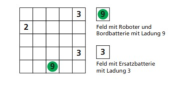
\includegraphics[width=0.8\textwidth]{Stromrallye_Feld.pdf}
    
    \caption{Ein Stromrallye Spielfeld
    \textit{\textcite{bwinfSpielfeld}
    }}
    \label{fig:stromrallye_spiel}
\end{figure}
\par
Bei dieser Aufgabe spielt das Spiel \textbf{Stromrallye} eine entscheidende Rolle.
In dem Spiel Stromrallye gibt es ein quadratisches Spielfeld mit Feldern.
Auserdem gibt es einen \textbf{Roboter}, welcher sich nach oben, unten, rechts und links bewegen kann, wenn er einen Schritt geht, verliert seine Batterie Akkuladung.
Wenn sein Akku leer ist, kann sich der Roboter nicht mehr bewegen.
Es gibt Ersatzbatterien auf dem Spielfeld mit unterschiedlichen Ladungen.
Wenn der Roboter auf ein Feld mit einer Ersatzbatterie kommt, \textbf{muss} dieser die Batterie mit der eigenen tauschen.
Die Aufgabe ist nun, fur ein Konstellation von Roboter und Ersatzbatterien, herauszufinden ob es moglich ist durch Bewegen des Roboters die \textbf{Ladestande} aller Batterien(Ersatzbatterien plus Roboters Batterie) auf \textbf{null} zu bringen und durch welche Schrittabfolge des Roboters dies moglich ist.
\textit{\textcite{bwinfSpielfeld}}
\subsubsection{Losungsidee}
Da das Ziel ist, den Ladestand aller Batterien auf 0 zu bringen, muss der Roboter sich zu den anderen Batterien bewegen.
Der einzige Weg, um die Ladung einer Batterie auf 0 zu bekommen, ist, indem man zu der Batterie geht und dann die Ladung der Batterie zu verbrauchen.
So muss der Roboter zu den anderen Batterien gehen. Zu jeder Batterie  die einen Ladestand hoher als null hat muss gegangen werden.
Dabei gibt es aber mehrere Batterien, zu denen der Roboter gehen kann.
Von diesen Batterien kann der Roboter wieder zu mehreren anderen Batterien laufen.
\par
\subsubsection{Kurzester Weg}
Auserdem ergibt es manchmal Sinn nicht den \textbf{kurzesten Weg} zu einer anderen Batterie zu gehen.
Manchmal ergibt es auch Sinn einen langeren Weg zu laufen. Dabei kann man fast alle Wege um eine \textbf{gerade Zahl verlangern} indem man hin und her lauft. Man kann kann einen Weg aber nicht um eine ungerade Zahl verlangern.
Wenn man einen Weg vom Roboter zu einer Ersatz-Batterie finden will, dann sind alle anderen Ersatz-Batterien Hindernisse, welche nicht begehbar sind.
\begin{figure}[h]
    \centering
    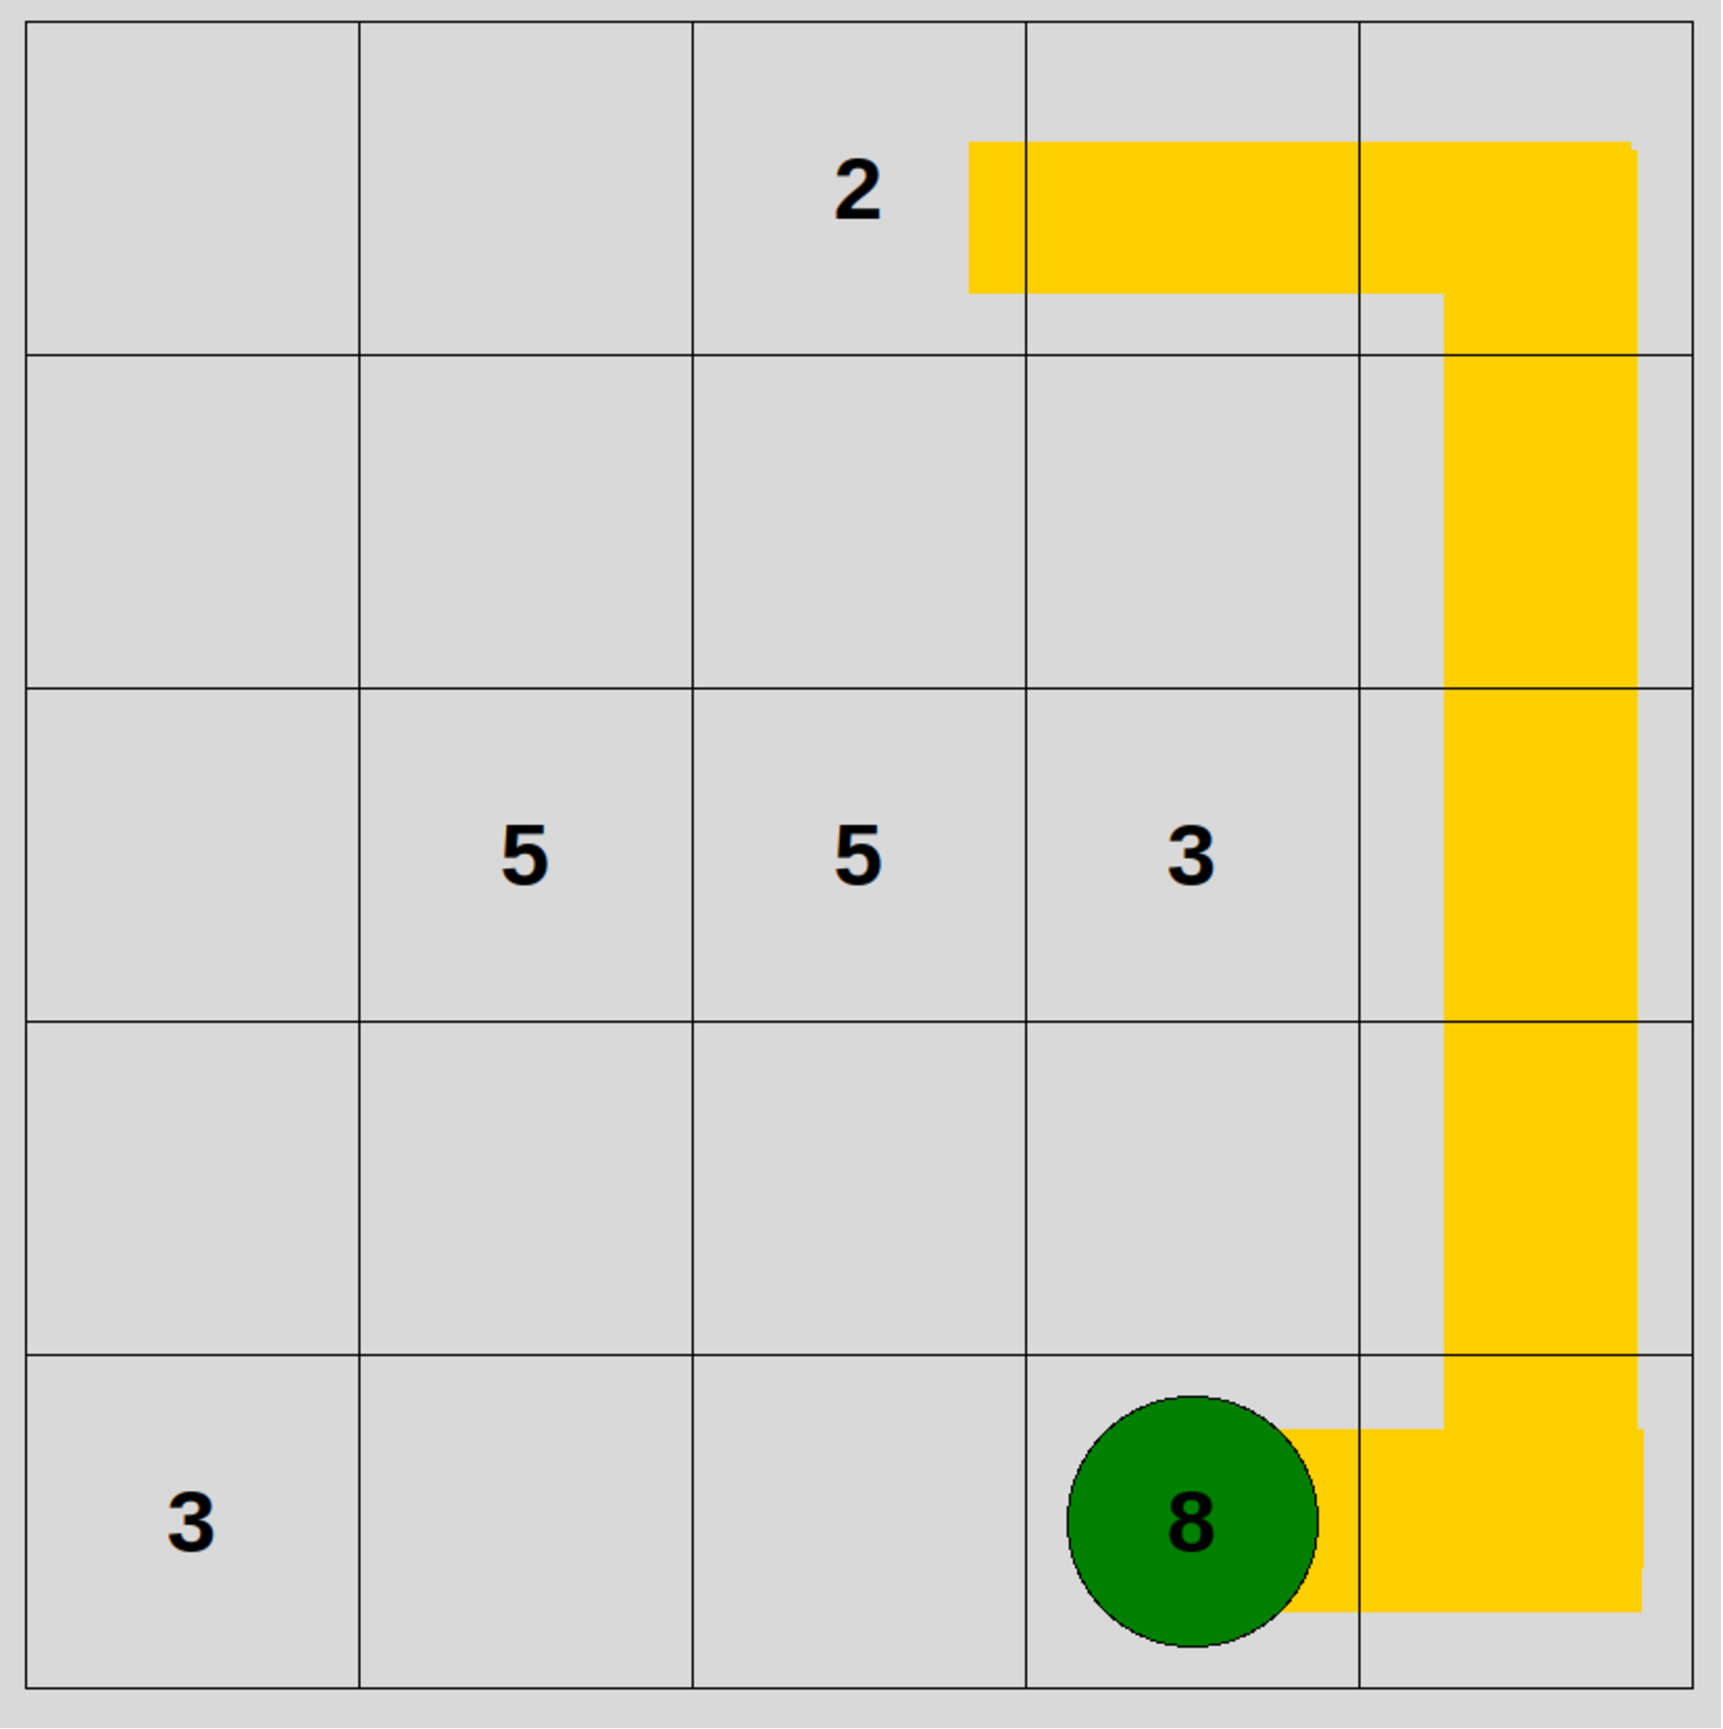
\includegraphics[width=0.9\textwidth]{shortest_w.pdf}
    \caption{Kurzester Weg vom Roboter zu einer Ersatz-Batterie}
    \label{fig:kurzester_weg}
\end{figure}
\par
In Abbildung \ref{fig:kurzester_weg} sieht man den kurzesten Weg vom Roboter zur Ersatz-Batterie mit der Ladung 2. Der kurzeste Weg ist mit der gelben Verfarbung gekennzeichnet. Der Roboter kann nicht den direkten Weg gehen, da die Ersatz-Batterien 5 und 3 den Weg versperren.



\paragraph{Weg Verlangern}

\begin{figure}[h]
    \centering
    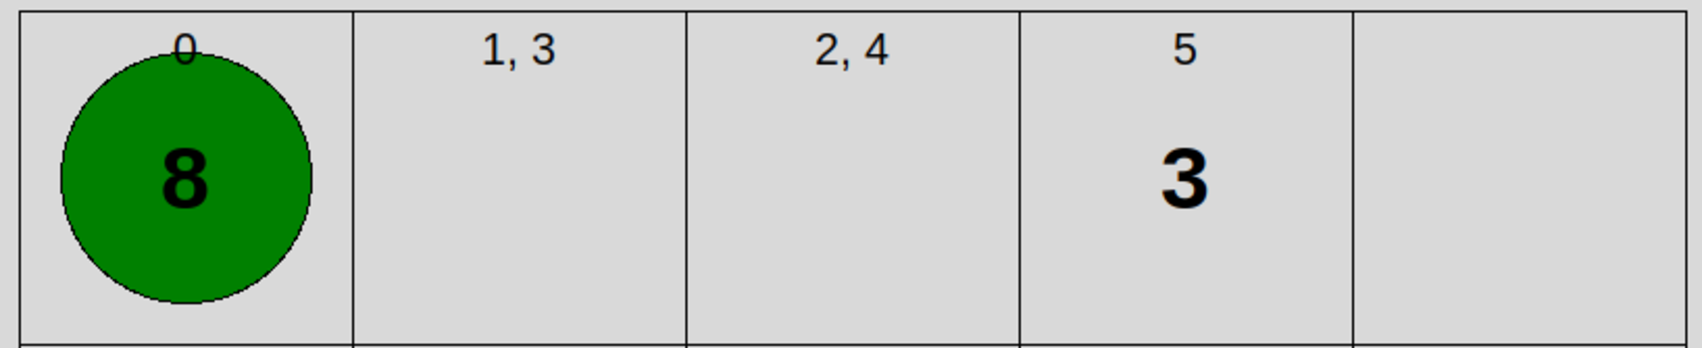
\includegraphics[width=0.9\textwidth]{weg_verlaengern_n.pdf}
    \caption{Weg Verlangern}
    \label{fig:weg_verlangern}
\end{figure}
In Abbildung \ref{fig:weg_verlangern} wird gezeigt, wie ein Weg verlangert werden kann. Die Zahlen zeigen, wann der Roboter dieses Feld besucht. In diesem Beispiel ist der kurzeste Weg 3 Schritte lang, wurde aber zu 5 Schritte verlangert. Der Weg kann auch weiter verlangert werden, indem noch ofter hin und her gelaufen wird.

\par
Die \textbf{Kurzesten Wege} vom Roboter zu den anderen Batterien werden durch \textbf{Breiten Suche} \cite{cormen} herausgefunden, dies ist \textbf{A-Stern} \cite{hart} vorzuziehen, da A-Stern nur den Weg von einem Knoten zu einem anderen berechnet, die Breiten Suche findet bei einer Durchfuhrung den kurzesten Weg zu allen anderen Knoten. \textbf{Djikstra} \cite{dijkstra} ist auch ein Algorithmus um den kurzesten Weg zu finden und findet auch nach einer Durchfuhrung den kurzesten Weg zu allen Knoten. \textbf{Breiten Suche} ist trotzdem die beste Wahl, da \textbf{Breiten} Suche die \textbf{Zeitkomplexitat}, $E$ = Kanten $V$ = Knoten $O(E + V)$ und \textbf{Djikstra} $O(V * log(V) + E)$ (wenn Djikstra mit Fibonacci-Heap verwendet wird). Somit ist die \textbf{Breiten Suche schneller als Djikstra}.

\paragraph{Der Graph}
Man kann das Spielfeld in einen Graphen umwandeln. Die Spielfelder sind die Knoten.
Es handelt sich um einen ungerichteten, ungewichteten Graphen, alle Konten sind in beide Richtungen begehbar und haben das Gewicht 1.
Wenn man versucht den kurzesten Weg vom Roboter zu einer Batterie zu finden, sind alle anderen Batterien Hindernisse, da man eine Batterie aufnehmen muss, wenn man auf ihr Feld geht. Deswegen sind im erzeugten Graph alle Felder mit Batterien, auser der Ziel-Batterie, nicht begehbar.
\begin{figure}[h]
    \centering
    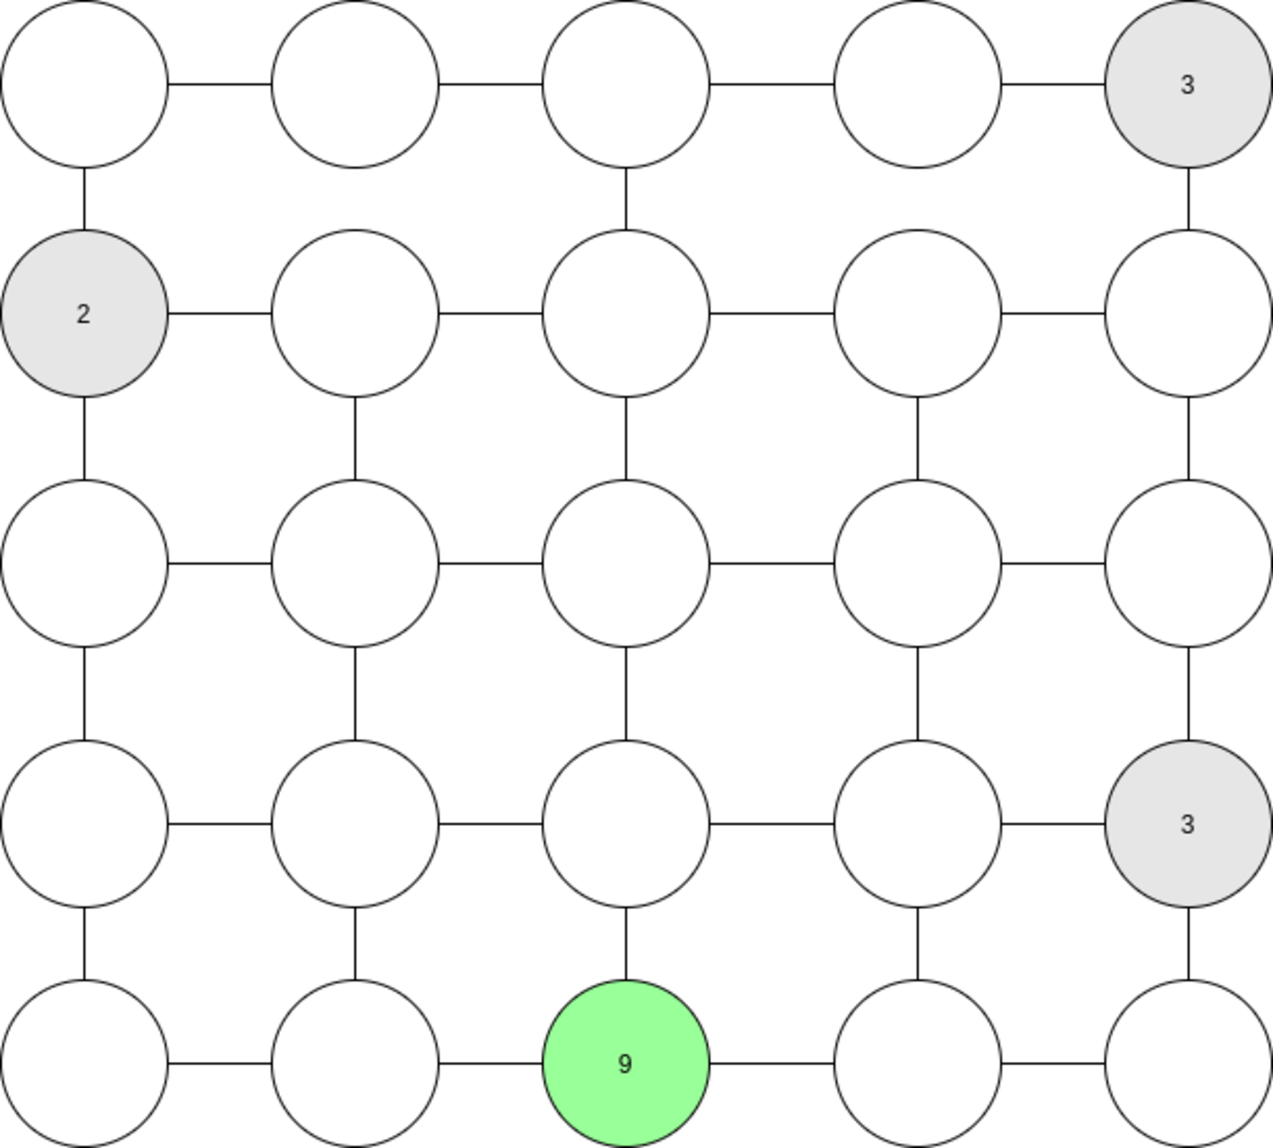
\includegraphics[width=0.5\textwidth]{graph_stromrallye.pdf}
    \caption{Das Stromrallye Spiel als Graph}
    \label{fig:graph_stromrallye}
\end{figure}
In Abbildung \ref{fig:graph_stromrallye}, sind die Ersatzbatterien mit grau gekennzeichnet, der Roboter mit grun.
Dies ist zum besseren Verstandnis.
In unserem Graphen, wird nicht gespeichert wie gros die Ladung der Ersatzbatterien ist, dies ist in der Grafik nur fur besseres Verstandnis so dargestellt.
Der Graph speichert, aber ob ein Feld (dies entspricht im Graphen einem Knoten) begehbar ist. Ersatzbatterien sind nicht begehbar, wenn man den Weg zu einer anderen Batterie finden will.

\newpage
\subsubsection{Erklarung Graph}
Ein Graph ist eine Datenstruktur.
Ein Graph besteht aus Knoten und Kanten.
Die Knoten sind mit Kanten miteinander verbunden.
Es gibt gerichtet und ungerichtete Graphen.
In gerichteten Graphen haben Kanten eine Richtung, in ungerichteten nicht.
Man kann von einem Knoten uber eine Kante zu einem anderen Knoten kommen usw..
In einem gewichteten Graphen haben Kanten zusatzlich ein Gewicht. Dies bedeutet, das ein bestimmtes Gewicht(oder Kosten) verwendet wird um von dem einen Knoten zum anderen zu kommen.
\begin{figure}[h]
    \centering
    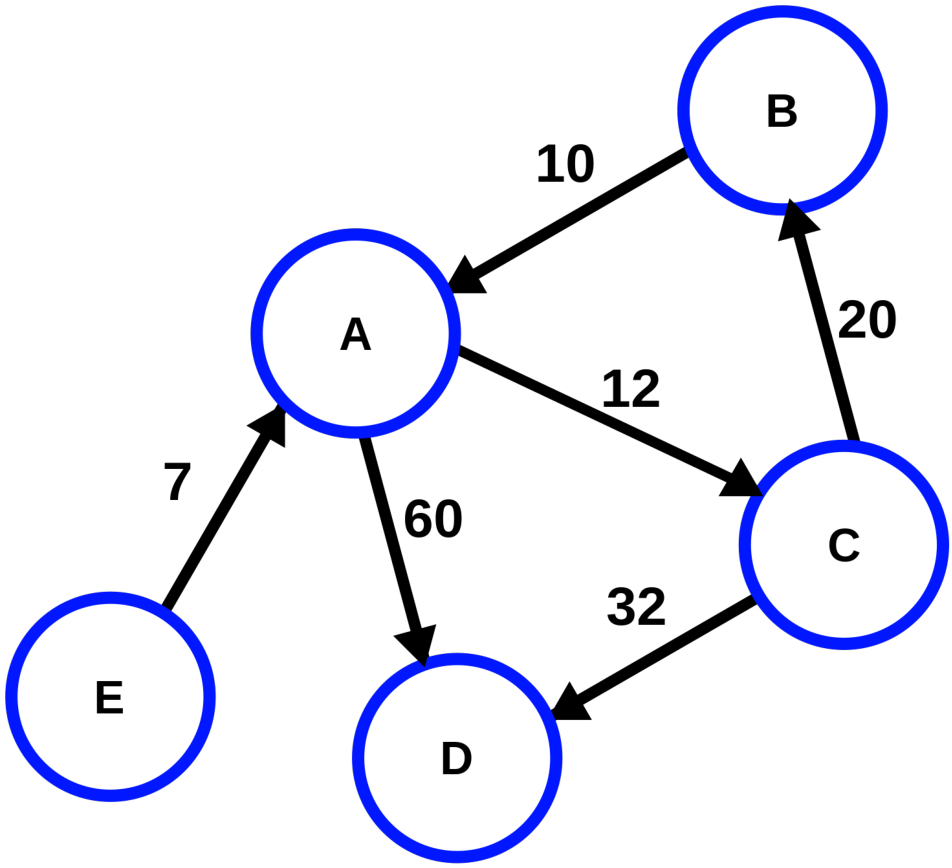
\includegraphics[width=0.5\textwidth]{graph.pdf}
    \caption{Ein Graph \textcite{wikipediaGraph}}
    \label{fig:graph}
\end{figure}

Beispielsweise in einem U-Bahn Netz sind Stationen die Knoten. Die Kanten sind U-bahn-Strecken, die Kosten der Kanten geben an, wie lange es braucht um mit der U-bahn diese Strecke zu fahren.
\begin{figure}[h]
    \centering
    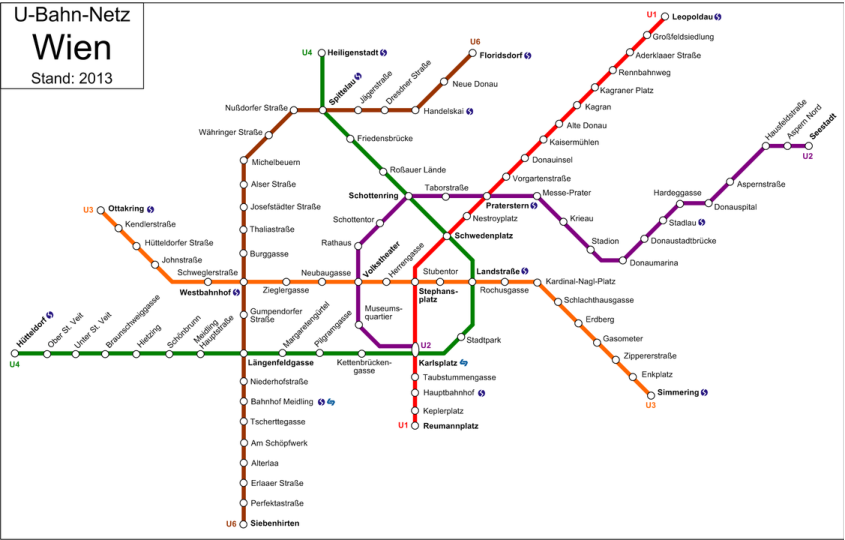
\includegraphics[width=0.9\textwidth]{u-bahn.pdf}
    \caption{Wiener U-bahn Netz \textcite{wikipediaUbahn}}
    \label{fig:u-bahn-netz}
\end{figure}



\subsubsection{Breiten Suche}
Bei der Breiten Suche startet man vom Startknoten und uberpruft dann alle Kinder, bzw. Nachbarn des Startknotens, ob sie der Zielknoten (oder eines der Zielknoten) sind.
Dies wird veranschaulicht in der Abbildung .
\begin{figure}[h!]
    \centering
    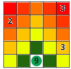
\includegraphics[width=0.4\textwidth]{Stromrallye_Feld_BFS.pdf}
    \caption{Schaubild des Spielfelds mit Breiten Suche berechnete kurzeste Wege. grun: 1 Schritt, gelb: 2 Schritte -> \textcite{bwinfSpielfeld}}
    \label{fig:bfs_stromrallye}
\end{figure}
Dies wird nun fur jeden Knoten rekursiv durchgefuhrt.
In einem Set (Erklarung in Kapitel \ref{sec:HashSet}) wird gespeichert welche Knoten bereits besucht worden sind und deswegen nicht nochmal besucht werden mussen.
Der Algorithmus terminiert wenn entweder Wege zu allen Zielknoten gefunden wurden oder alle Felder besucht wurden(es kann sein, dass es zu einem Zielknoten gar keinen Weg gibt).

Die Breiten Suche funktioniert nur in einem Graph ohne Kanten Kosten, bzw. alle Kanten Kosten mussen gleich sein. In unserem Fall ist diese Bedingung gegeben, deswegen konnen wir die Breiten Suche verwenden um den kurzesten Weg zu finden.
In unserem Graph hat jede Kante den Kosten 1, dar der Roboter eine Energieladung verbraucht wenn dieser einen Schritt lauft.
\par
In unserem Fall kann die breiten Suche auch bereits dann abgeschlossen werden, wenn alle Felder in der Reichweite des Roboters besucht wurden.
\subsubsection{Djikstra}
Der Djikstra Algorithmus funktioniert an sich ahnlich der Breiten Suche. Zusatzlich sortiert der Djikstra Algorithmus die Knoten nach Kosten und besucht den Knoten zuerst zu dem ein Weg mit geringsten Kosten gefunden wurde.
\\
Dies bringt in unserem Fall nichts, dar alle Knoten die gleichen Kosten haben und zwar 1. Das sortieren der Knoten verbraucht aber zusatzliche Zeit, welches den Djikstra Algorithmus langsamer macht als die Breiten Suche.
\subsubsection{A-Stern}
Bei A-Stern wird zusatzlich noch eine Heuristik verwendet, um den best-moglichen Pfad zuerst zu verwenden.
In unserem Fall ware so eine Heuristik, wie weit der Knoten vom Zielknoten entfernt ist. 
Im A Stern Algorithmus werden dann Knoten die naher am Zielknoten sind zuerst besucht.
Dies macht den A Stern Algorithmus deutlich schneller als Djikstra und Breiten Suche.
Die breiten Suche kann man nochmal stark verbessern, dadurch, dass man eine Heuristik verwendet.
Die Wahrscheinlichkeit, dass der schnellste Weg in der Richtung in der der Zielort liegt, ist viel wahrscheinlicher, dies nutzt man bei A Stern clever, um den Algorithmus wesentlich schneller zu machen.

\subsubsection{Kurzester Weg-Fazit}


Die Breiten Suche ist am schnellsten, da diese mit einer Durchfuhrung die kurzesten Wege zu allen Ziel-Knoten findet. Auserdem keine zusatzliche Zeit durch sortieren der Knoten verbraucht.



\par

\subsubsection{Kürzester Weg Laufzeitanalyse}
In unserem ungerichteten Graphen ist der Weg von a ->b, der gleiche wie b -> a, umgedreht.
Beispiel: \\
Im Graphen mit den Kanten:\\
a <-> b \\
b <-> c\\
Ist der schnellste Weg von a nach c (a, b, c). \\
Der Weg von c nach b, ist (c, b, a). \\
Damit die Breiten Suche nicht immer wieder neu ausgeführt wird, speichern wir unsere vorherigen Ergebnisse in einer HashMap. 
Der kürzeste Weg wird immer von Roboter zu den Ersatzbatterien berechnet. Der kürzeste Weg wird nur berechnet wenn der Roboter auf einer Ersatzbatterie steht, oder bei der Startposition.
Also gibt es  \textbf{Anzahl-Ersatzbatterien + \texttt{1}} außer wenn der Roboter sich beim Start schon auf einer Ersatzbatterie befindet).
Also wenn $e$, die Anzahl der Ersatzbatterien (+1) ist. \\
Dann müssen maximal $e * (e-1)$ viele Wege berechnet werden.
Bei der Ausführung von Breiten Suche werden, direkt von einem Start Wege zu allen Zielen gefunden.
Deswegen muss die Breiten Suche maximal $e$ oft ausgeführt werden.

Da die Breiten Suche $O(E+V)$ lange dauert, kommen wir so auf eine worst-case Laufzeitkomplexität von $O(e * (E + V))$.

\subsubsection{Der Weg zu sich selbst}
Von einer Ersatzbatterie kann es auch Sinn machen wieder zu sich selbst zu laufen,
dabei ist der Weg zu sich selbst immer 2 Schritte lang, es kann aber auch sein, dass es keinen Weg zu sich selbst gibt.
\begin{figure}[h]
    \centering
    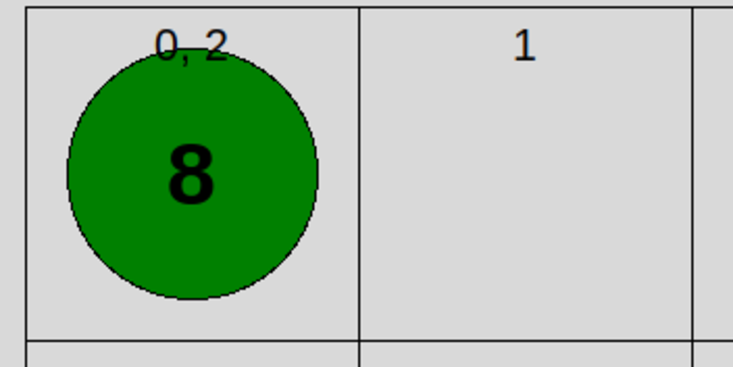
\includegraphics[width=\textwidth]{way_to_self.pdf}
    \caption{Weg zu sich selbst}
    \label{fig:way_to_self}
\end{figure}

\newpage
\subsubsection{Der Weg ins Nichts}
Wenn alle Batterie-Ladungen 0 sind, nur der Roboter noch Ladung hat, muss dieser seine Ladung verlieren. Es kann aber vorkommen, dass dies nicht funktioniert, da alle Wege von anderen Batterien versperrt sind. Deswegen muss dies uberpruft werden.
\begin{figure}[h]
    \centering
    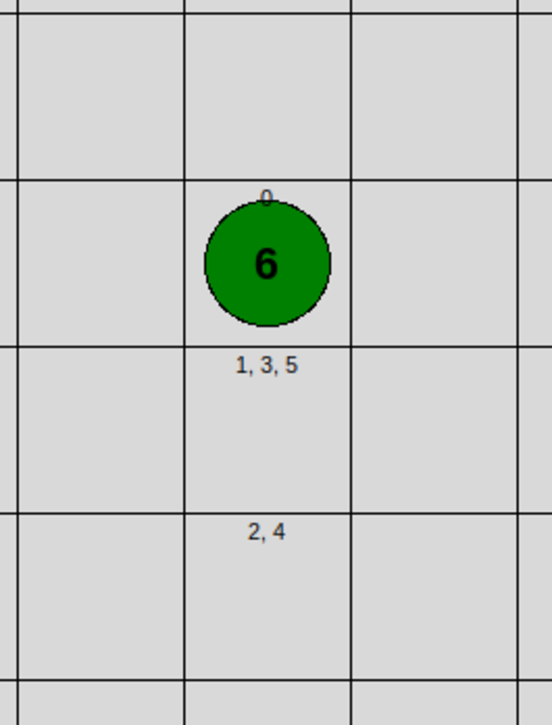
\includegraphics[width=0.8\textwidth]{way_ins_nothing.pdf}
    \caption{Weg ins nichts! Benutzung der ganzen Batterie-Ladung}
    \label{fig:way_to_nothing}
\end{figure}

\subsubsection{Ersatzbatterien}

Der \textbf{Roboter} kann von einer Position mit einem bestimmten Ladestand unterschiedliche Ersatzbatterien erreichen. Nachdem der Roboter zu einem dieser Ersatzbatterien gelaufen ist, kann dieser von dort wieder zu verschiedenen Ersatzbatterien laufen.
\par
Wie bereits beschrieben, kann es aber auch Sinn machen, dass der Roboter nicht den kurzesten Weg zu einer Ersatzbatterie zu gehen. Da ein Weg immer um eine gerade Zahl verlangert werden kann, mussen diese Moglichkeiten auch durchgegangen werden.
Also wenn der kurzesten Weg $w$ lang ist und der Roboter $b$ Batterieladung hat, dann sind $(a(n)  = max(w + 2n, b))$ $n >= 0$ mogliche Langen an Wegen.
So gibt es vom Roboter zu einer Ersatzbatterie $(b - w) / 2$ mogliche Weglangen.
\\
Zum Beispiel:
Wenn der Roboter mindestens 5 Schritte zu einer Batterie braucht und gerade 9 Ladung hat. Dann sind 5, 7, 9 mogliche Anzahl Schritte um zur Batterie zu kommen.
\\
Der kurzeste Weg ist 5 Schritte lang und der Roboter hat die Batterie-Ladung 9, da der Weg um eine gerade Zahl verlangert werden kann, sind auch 7 und 9 moglich.

\subsubsection{Moglichkeiten}

Diese \textbf{Moglichkeiten} des Roboters werden in einem \textbf{Baum} gespeichert.
Dabei werden in den \textbf{Knoten} der Spielstand(Position und Ladestand der Ersatzbatterien und des Roboters) und in den \textbf{Kanten} die Schritte und Anzahl an Schritten, welche der Roboter laufen muss, um den Spielstand $a$ zu Spielstand $b$ zu verandern.
Dabei ist Spielstand $b$ auch wieder ein Spiel welches gelost werden kann.
\\
Um von Spielstand $a$ zu Spielstand $b$ zu kommen muss der Roboter eine Schrittabfolge laufen.
Der Losungs Spielstand, besteht aus einem leeren Roboter und nur Leeren Batterien.


\par
\subsubsection{Baum}
Ein Baum ist eine Art von Graph in welchem ein Knoten Kinder hat. Diese Kinder sind untereinander nicht verbunden.
Knoten haben immer nur einen Eltern-Knoten. Das Eltern-Knoten muss eine Ebene oben druber sein. Die Kinder eines Knotens sind immer eine Ebene unten drunter.


\subsubsection{Moglichkeiten-Baum}
Um nun herauszufinden ob es eine Losung gibt und welche diese ist, wird der Weg herausgesucht, welcher die grosten summierten Anzahl an Schritten hat.
Also einer der Wege mit denen der Roboter die meisten Schritte zurucklegen kann.
Wenn die Anzahl der Schritte, der Summe der Batterieladungen (Ersatzbatterien und Roboter) entspricht, ist dies eine korrekte Losung um den Ladestand aller Batterien auf 0 zu bringen.
Abbildung:
Losung mit grun markiert
    RU : Batterie rechts unten auf dem Spiel
    RO: Batterie rechts oben auf dem Spiel
    LO: Batterie links oben
    RS: Roboters Startposition
\par
\newpage

\begin{figure}[htpb]
    \centering
    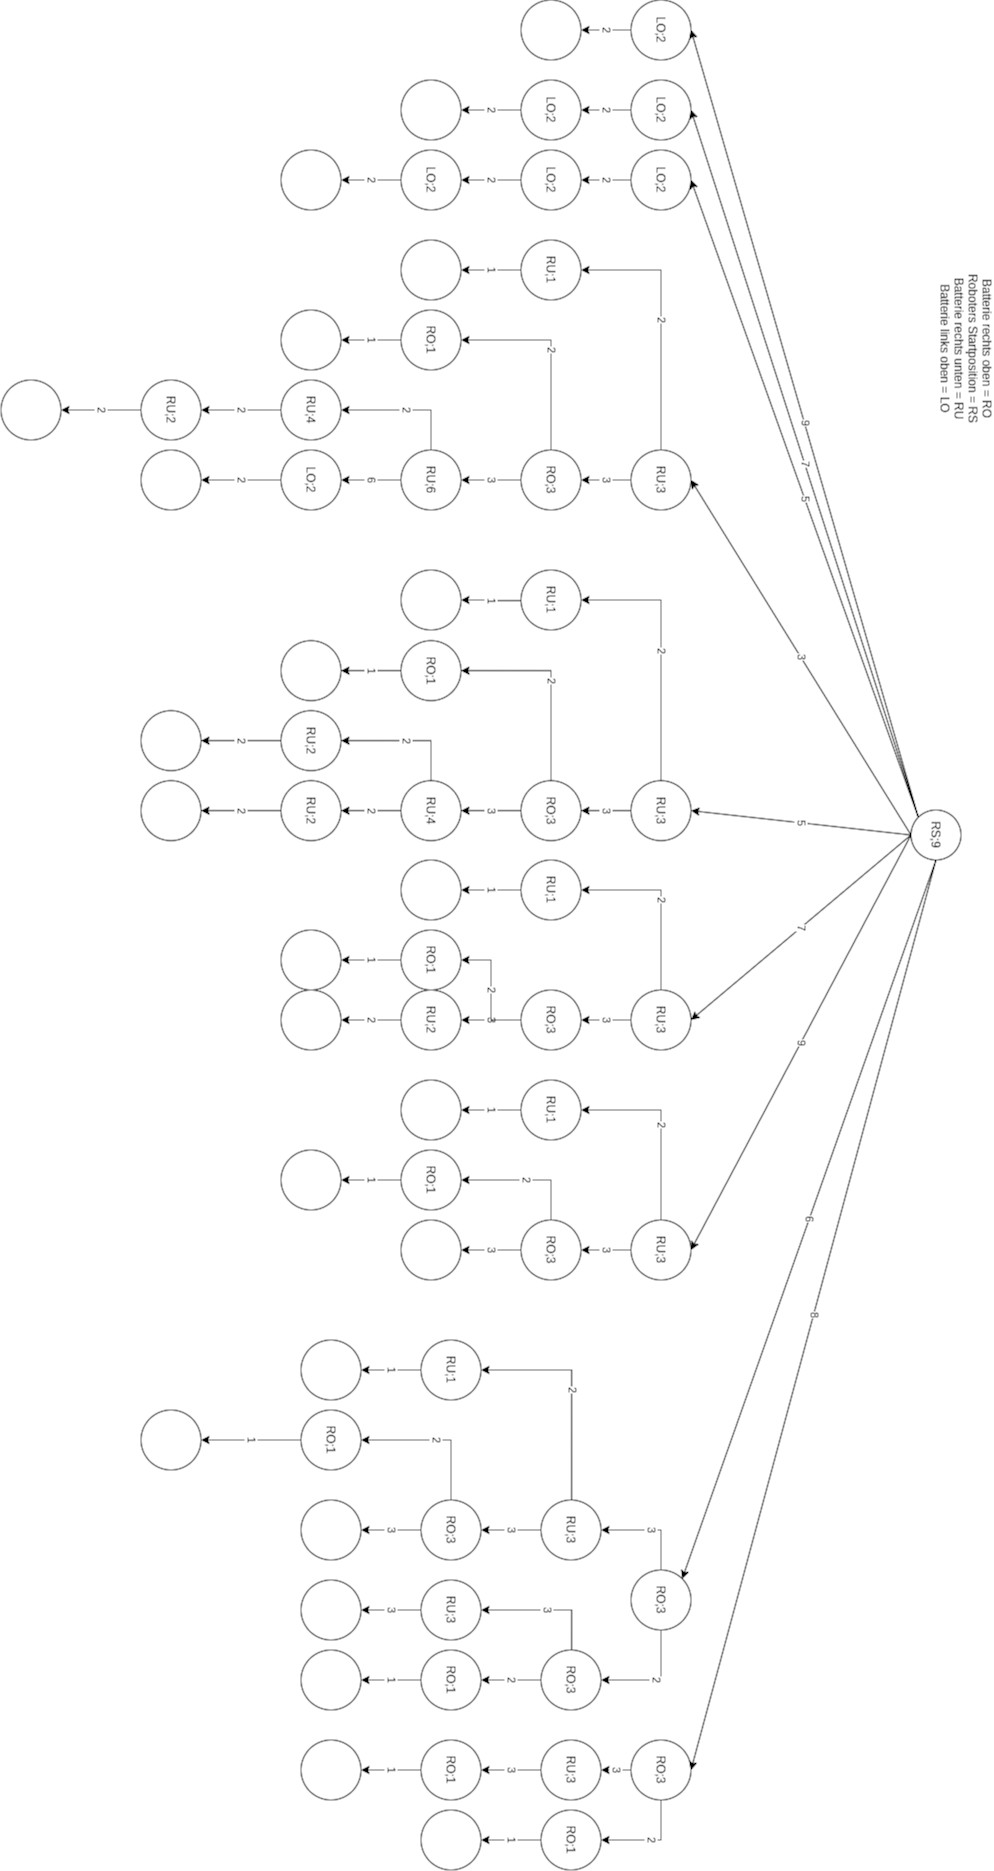
\includegraphics[width=0.6\textwidth]{rotated_baum_yeah.jpg}
    \caption{Schaubild des Moglichkeiten-Baums
    }
    \label{fig:moeglichkeiten_baum}
\end{figure}

\newpage

\subsubsection{insgesamte Laufzeitanalyse}
Größen sind:
\begin{itemize}
    \item Größe des Spielfelds
    \item Anzahl Batterien
    \item Summe der Ladungen an Batterien
\end{itemize}

Die Laufzeit meines Algorithmus ist von all diesen genannten Größen abhängig.
Desto größer das Spielfeld, desto länger braucht mein Programm.
Desto mehr Batterien, desto Länger braucht der Algorithmus.
Desto mehr Ladung, desto länger braucht mein Programm.
\par
Am abhängigsten ist mein Algorithmus, aber von der Anzahl an Batterien. Aus dem folgenden Grund, dass sich der Möglichkeiten Baum sehr stark vergrößert.
Die Zahl an Knoten im Baum nimmt stark an, wenn es eine höher Anzahl an Batterien gibt.
\par
Der worst-case für meinen Algorithmus ist, dass sich auf jedem Feld des Spielfelds eine Batterie befindet, mit der Ladung 1. Dies führt zu einer Zeitkomplexität von $O(4)^L$; wenn $L$ die Gesamt Summe der Batterien ist, welche dann äquivalent zur Anzahl Felder ist, also der quadrierten Größe. Daher gilt auch $O(4^(s*s))$; $s$für size entspricht der Größe des Spielfelds.
Die 4 aus dem Grund, dass es 4 Richtungen gibt, in welche sich der Roboter bewegen kann.
\par
Die Zeit für das Berechnen, der kürzesten Wege, fällt bei Spielen mit vielen Batterien nicht so stark ins Gewicht.\par
Die Breiten Suche braucht $O(e * (E + V))$, $e$ Anzahl Ersatzbatterien, $E$ Edges, $V$ gleich Vertices. Jeder Knoten hat maximal 4 Kanten(bzw. Nachbarn), also $O(E) = O(V)$, $O(e * (E+V)) = O(e * V)$. In unserem worst-case Szenario beschrieben im vorherigen Absatz, entspricht die Anzahl der Knoten, der Anzahl an Feldern, also $e=s*s$; $s$ für size ist die Größe des Spielfelds.
$V$ wiederum entspricht ebenfalls $s*s$. Daher kommen wir insgesamt auf $O(s*s*s*s)$,
also $O(s^4)$. Da $e$ = $s * s$. Können wir auch sagen $O(e^2)$. Also ist die Laufzeit der Breiten Suche quadratisch zur Anzahl Batterien.
Die Laufzeit für den Möglichkeiten Baum ist wesentlich größer.
Sie ist $O(4^(s*s))$ oder $O(4^e)$.
Beide Laufzeiten addiert: $O(4^e) + O(e^2)$ = $O(4^e)$
\textbf{Die insgesamte worst-case Laufzeit ist:}
\begin{itemize}
\item In Abhängigkeit der Anzahl Batterien($e$) => \texttt{$O(4^e)$} \\
\item In Abhängigkeit der Größe des Spielfelds($s$) => \texttt{$O(4^(s*s))$}
\item In Abhängigkeit der Größe< des Spielfelds($L$) => \texttt{$O(4^L)$}
\end{itemize}
\subsubsection{Umsetzung}
Der Algorithmus wird in Python(Version 3.7) implementiert.


\newpage
\subsubsection{UML-Klassen-Diagramm}
\begin{figure}[h]
    \centering
    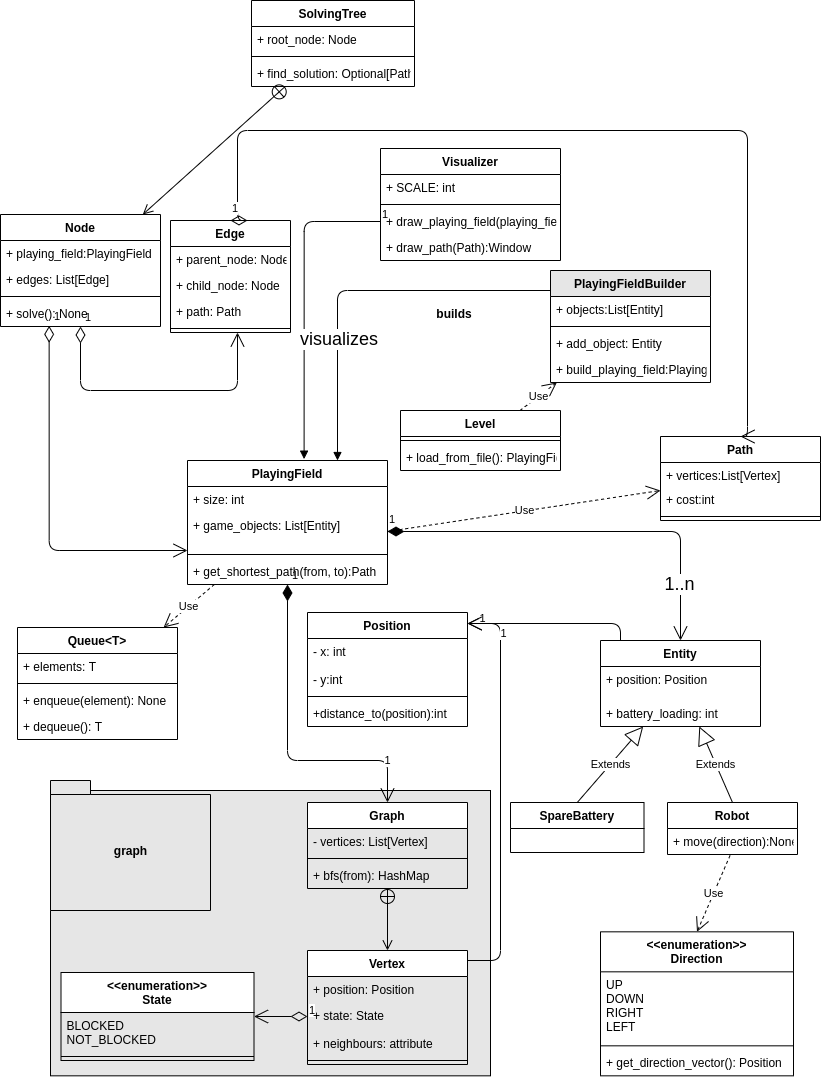
\includegraphics[width=0.85\textwidth]{uml_diagramm.png}
    \caption{UML Klassen Diagramm}
    \label{fig:uml}
\end{figure}
\newpage

\begin{classInformation}{SolutionTree}
\addDescription{
Der \textit{SolutionTree} lost ein Spielfeld,
er speichert die \textit{root\_node} (siehe \ref{sec:Node} auf Seite \pageref{sec:Node}.)
Diese \textit{root\_node} hat wiederum Kind-Knoten, welche auch wieder Kind-Knoten haben usw. .
Mit der Funktion \textit{find\_solution} wird eine Losung fur das entsprechende Spielfeld (das Spielfeld wird nicht im \textit{SolutionTree} selbst gespeichert, aber in der \textit{root\_node} ) gefunden, falls eine existiert.}

\begin{relations}
\hasObjects{Node}{sec:Node}
\end{relations}


\begin{classAttributes}
\addAttribute{-}{root\_node}{Node}{Die \textit{root\_node} ist der oberste Knoten im \textit{SolutionTree}, sie hat selbst wieder Kind-Knoten welche wieder Kind-Knoten haben usw.}
\end{classAttributes}

\begin{classMethods}
\addMethod{+}{find\_solution()}{Optional[Path]}{Die \textit{find\_solution} Methode findet einen Pfad, welcher das Spielfeld, der \textit{root\_node} lost, falls es losbar ist.}
\end{classMethods}
\end{classInformation}

\begin{classInformation}{Node}
\addDescription{Die \textit{Node}-Klasse ist Teil des \textit{Solution Tree} (siehe \ref{sec:SolutionTree} auf Seite \pageref{sec:SolutionTree}) . Auserdem speichert sie einen Spielstand des Stromrallze. Die \textit{Node} hat Kanten zu allen moglichen Knoten mit Spielstanden, welche durch des Bewegen vom Roboter zu einer Ersatzbatterie moglich sind.}
\begin{relations}
\item ist Teil vom \textit{SolutionTree} (siehe \ref{sec:SolutionTree} auf Seite \pageref{sec:SolutionTree})
\hasObjects{Edge}{sec:Edge}
\hasObjects{PlayingField}{sec:PlayingField}
\end{relations}
\newpage
\begin{classAttributes}
\addAttribute{-}{edges}{List[Edge]}{Die \textit{edges} sind die Kanten zu den Kind-Knoten der \textit{Node} (siehe \ref{sec:Edge} auf Seite \pageref{sec:Edge})}.
\addAttribute{-}{playing\_field}{PlayingField}{Das \textit{playing\_field} ist der Spielstand dieses Knotens.}
\end{classAttributes}


\begin{classMethods}
\addMethod{+}{solve()}{None}
{
Die \textit{solve()} Funktion, lost den Spielstand des Knotens (\textit{playing\_field}). Dabei ruft die \textit{solve} Funktion rekursiv, wieder solve fur alle Kind-Knoten des Knotens auf (siehe Pseudocode).
}
\end{classMethods}
\begin{pseudocode}
SOLVE(NODE):
    paths = getPathsToSpareBatteries()
    for i=0 to paths.length:
        newNode = Node()
        NODE.addEdge(Edge(NODE, newNode, paths[i]))
        SOLVE(newNode)
\end{pseudocode}
\end{classInformation}


\begin{classInformation}{Edge}
\addDescription{Die \textit{Edge} Klasse ist die Kante welche Knoten im \textit{SolutionTree}(siehe \ref{sec:SolutionTree} auf Seite \pageref{sec:SolutionTree}) miteinander verbindet.
Es wird der Pfad gespeichert, welcher der Roboter laufen muss um den Zustand des Spielfelds von Eltern- zu Kind-Knoten zu verändern.}
\begin{relations}
\item ist Teil des \textit{SolutionTrees}
\hasObjects{Node}{sec:Node}
\hasObjects{Path}{sec:Path}
\end{relations}

\begin{classAttributes}
\addAttribute{-}{path}{Path}{Die \textit{path}-Variable, gibt an, welcher Pfad der Roboter gehen muss um den Zustand des Spielfelds vom Eltern-Knotens-Spielstand zum Kind-Knotens-Spielstand zu verändern.}
\addAttribute{-}{parent\_node}{Node}{Die \textit{parent\_node}  speichert den Eltern-Knoten}
\addAttribute{-}{child\_node}{Node}{Die \textit{child\_node}  speichert den Kind-Knoten}
\end{classAttributes}
\noMethods
\end{classInformation}

\begin{classInformation}{Entity}


\addDescription{
Die \textit{Entity} Klasse, beinhaltet alle Dinge, welche Roboter und Ersatzbatterie gemeinsam haben.
Roboter und Ersatzbatterie erben beide von Entity.
Beide haben eine Position und einen Ladestand.
}
\begin{classAttributes}
\addAttribute{-}{position}{Position}{Die \textit{position} gibt die Position der Entitz auf dem Spielfeld an}
\addAttribute{-}{battery\_-loading}{int}{Der aktuelle Batterie-Ladestand der Batterie}
\end{classAttributes}
\noMethods
\end{classInformation}

\begin{classInformation}{Position}
\addDescription{Die \textbf{Position} Klasse, speichert die Position der entitys(Roboter, Ersatzbatterien).
Da wir uns im 2 dimnsionalen Raum befinden, besteht die Position aus x und y Koordinate, welche Attribute der Position Klasse sind.\\
Dabei habe ich ein Kordinatensystem gewahlt, indem %TODO
oben links ist.
Nach unten steigt y, nach rechts steigt x.
Die Positions Klasse konnte man auch als Vektor bezeichnen.
Sie implementiert die gängigsten Vektor Funktionenen, darunter (plus, minus, länge des vektors, multiplikation ...)

}

\begin{classAttributes}
\addAttribute{-}{x}{int}{Die x-Koordinate der Position.}
\addAttribute{-}{y}{int}{Die y-Koordinate der Position.}
\end{classAttributes}

\begin{classMethods}
\addMethod{+}{manhattan\_-distance(other\_position)}{int}{manhattan distanz zur anderen Position. Die Manhattan Distanz wird folgendermaßen berechnet, $|x1 - x2| + |y1 - y2|$.
}
\end{classMethods}

\end{classInformation}

\begin{classInformation}{Roboter}
\addDescription{Der Roboter erbt von der Entity Klasse.
Zusatzlich hat der Roboter, aber noch Methoden um sich zu bewegen und um seine Batterie mit einer Ersatzbatterie auszutauschen.}
\\
\textbf{wichtige Attribute:}
\\
erbt die Attribute \textit{position} und \textit{battery\_loading} von \textit{Entity}

\begin{classMethods}
\addMethod{+}{move(direction)}{None}{Der Roboter kann sich bewegen.}
\addMethod{-}{change\_-battery()}{None}{Der Roboter wechselt die Batterie, mit der unter sich liegenden Ersatzbatterie. Die Methode ist \textit{privat} und wir vom Roboter aufgerufen, wenn er sich auf ein Feld mit einer Ersatzbatterie bewegt.}
\end{classMethods}
\end{classInformation}
\newpage
\begin{classInformation}{Enum-Directions}
\addDescription{Das Enum Description, gibt die vier Richtungen (oben, unten, rechts, links) an, in welche sich der Roboter auf dem Stromrallye-Spielfeld bewegen kann.}
Die 4 verschiedenen Werte, welcher das Enum Directions haben kann sind:
\textbf{Directions.UP}\\
\textbf{Directions.DOWN}\\
\textbf{Directions.LEFT}\\
\textbf{Directions.RIGHT}\\

\begin{classMethods}
\addMethod{+}{get\_direction\_-vector()}{Position}{Die Methode getdirectionvector gibt, den entsprechenden Richtungsvektor der Richtung zurück- UP => (0, -1)- DOWN => (0, 1)- RIGHT => (1, 0) - LEFT => (-1, 0).
In diesem Fall ist unsere Positions-Klasse, der Richtungsvektor
}
\end{classMethods}
\end{classInformation}
\begin{classInformation}{SpareBatterie}
\addDescription{Die Ersatzbatterie(SpareBattery) erbt von der Entity-Klasse. Da sie sich nicht bewegen kann und auch sonst nichts machen kann, hat diese keine besonderen Attribute oder Funktionen.}

\textbf{wichtige Attribute:}\\
erbt \textit{position}und \textit{battery\_loading} von \textit{Entity}
\noMethods
\end{classInformation}

\begin{classInformation}{Spielfeld}
\addDescription{Die Spielfeld Klasse beinhaltet alle Objekte des Spiels. Sie speichert die Elemente des Spiels. Außerdem auch das Spielfeld als Graphen. Sie hat eine Größe, da sie quadratisch ist, wird nicht zwischen Länge und Breite unterschieden.
}
\newpage
\begin{classAttributes}
\addAttribute{-}{size}{int}{Die Größe des Spielfelds}
\addAttribute{-}{game\_objects}{List[Entity]}{Die Liste aller Objekte, die auf dem Spielfeld sind.}

\end{classAttributes}
\begin{classMethods}
\addMethod{+}{get\_shortest\_-path(-from:Position, to:Position)}{Path}{Findet den kürzesten Weg auf dem Spielfeld von einer Position zu einer anderen, ohne andere Ersatzbatterien aufzusammeln außer des Ziels.}
\end{classMethods}

\end{classInformation}

\begin{classInformation}{Graph}
\addDescription{Die Graph Klasse, entspricht einem normalen Graphen in der Informatik. Es ist ein ungerichteter, ungewichteter Graph, weswegen es auch keine Kanten als Objekte gibt, auch keine Klasse, da alle Kanten Kosten 0 haben.
Stattdessen speichert jeder Knoten(Vertex), die Nachbar Knoten(Vertices).
Der Graph speichert alle Knoten in einer Liste.}

\begin{classAttributes}
\addAttribute{-}{vertices}{HashMap-[Position,- Vertex]}{Alle Knoten des Graphen werden in der HashMap \textit{vertices} gespeichert. Es wird eine HashMap verwendet, da man bei solcher nur konstante Zeit O(1) benötigt um ein Knoten an einem Punkt zu bekommen. Eine weitere Alternative ist ein 2-dimensionales Array, bei dem an Stelle vertices[x][y] -> der Knoten der Position x y ist.}
\end{classAttributes}
\begin{classMethods}
\addMethod{+}{bfs(from, to)}{HashMap[Vertex, Path]}{Führt die breiten Suche (engl. \textbf{b}readth \textbf{f}irst \textbf{s}earch) aus.}
\end{classMethods}
\end{classInformation}

\begin{classInformation}{Vertex}
\addDescription{Die Vertex-Klasse, ist ein Knoten des Graphen. Der Knoten kennt seine nachbar Knoten und hat eine Position.}
\begin{classAttributes}
\addAttribute{-}{position}{Position}{Position auf dem Spielfeld.}
\addAttribute{-}{neighbours}{List[Vertex]}{Nachbarknoten}
\end{classAttributes}
\begin{classMethods}
\addAttribute{+}{add\_neighbour}{None}{Fügt einen Knoten als Nachbar hinzu.}
\end{classMethods}
\end{classInformation}



\newpage
\subsubsection{Losungen}


Eingabe:
\texttt{ \\
5 \\
3,5,9 \\
3 \\
5,1,3 \\
1,2,2 \\
5,4,3 \\
}
\par
Erklarung:

Die Dateien enthalten jeweils ein Spielbrett mit den darauf verteilten Batterien und dem Roboter.

In der ersten Zeile ist Grose des Spielbretts angegeben,
in der zweiten Zeile sind die Koordinaten des Roboters und die Ladung seiner Batterie und
in der dritten Zeile ist die Anzahl der restlichen auf dem Spielbrett verteilten Batterien angegeben.
Ab der vierten Zeile ist in jeder Zeile eine Batterie angegeben, also Ihre Koordinaten und ihre Ladung.
Dabei sind die Angaben zu den Koordinaten und der Ladung der Batterien und des Roboters als drei kommagetrennte Werte in der Form "x,y,ladung" geschrieben.
\textcite{bwinfMaterial}.

\begin{figure}[htbp]
    \centering
    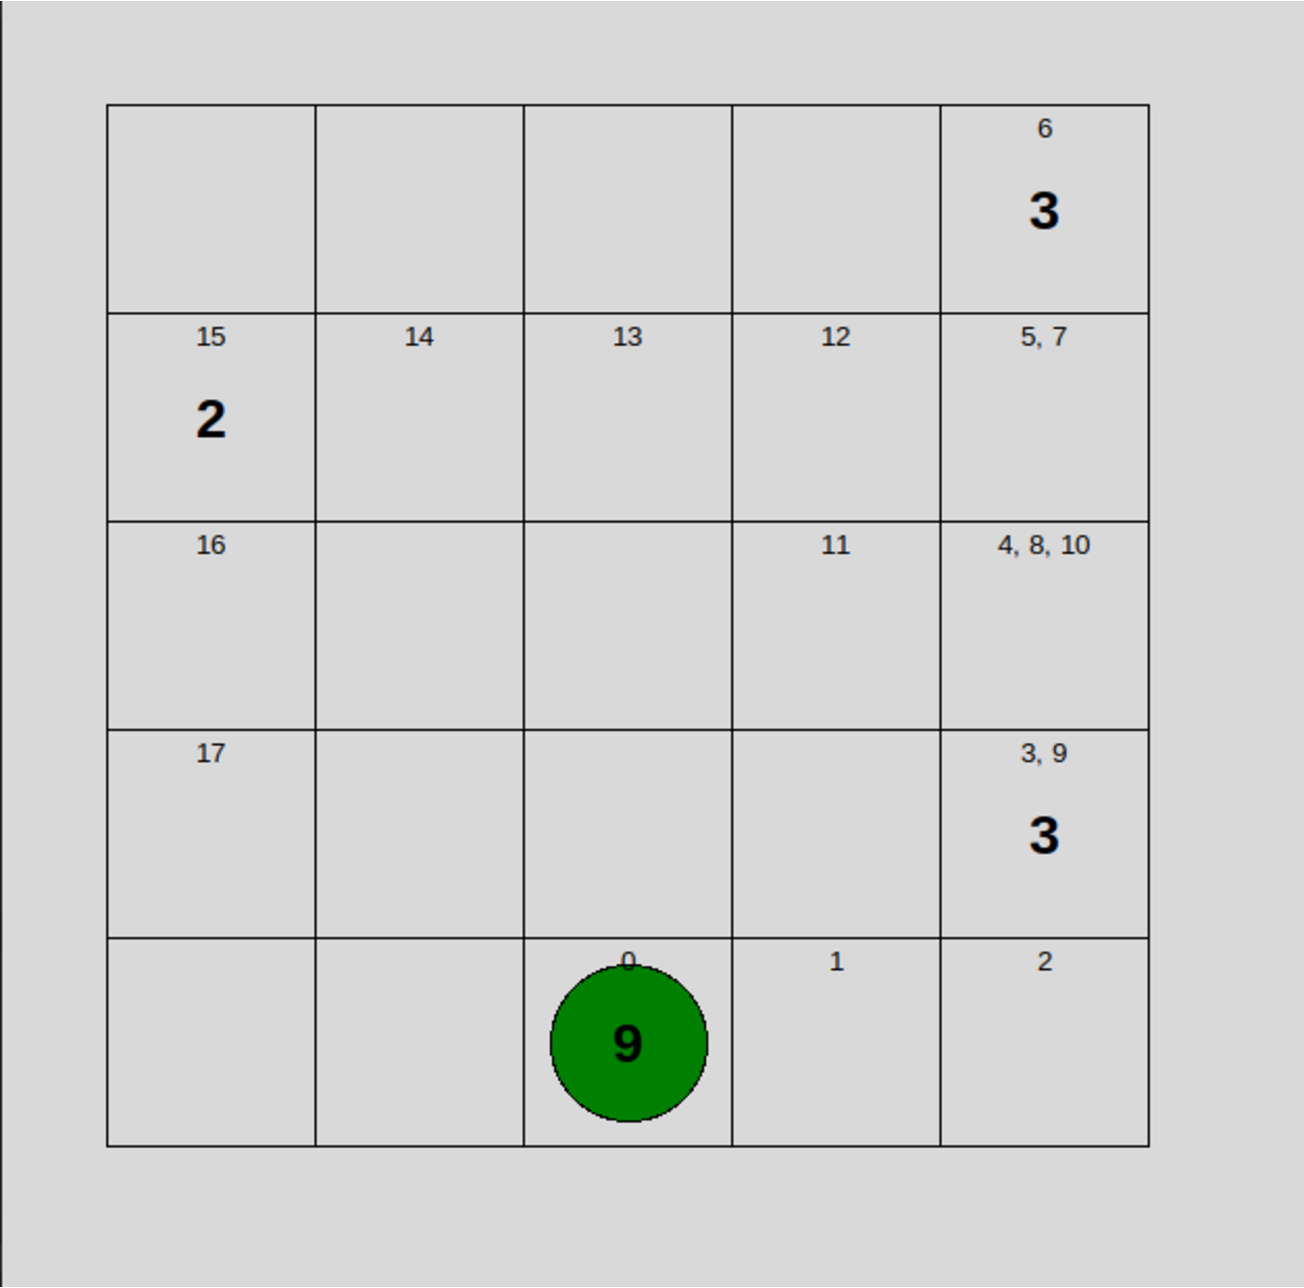
\includegraphics[width=0.7\textwidth]{Solution.pdf}
    \caption{Die Lösung des Stromrallye-Spiels}
    \label{fig:loesung1}
\end{figure}
\newpage
In Abbildung \ref{fig:loesung1} sieht man die Losung des BWinf Stromrallye Spiels. Die Zahl 9 mit dem grunen Kreis drumherum ist der Roboter, mit der Ladung 9.
Die Ersatzbatterien, sind die Fett gedruckten Zahlen in der Mitte der Felder, die Zahl zeigt die Ladung der Ersatzbatterien, beim Start an.
Die Ladung des Reboters und der Ersatzbatterien verandert sich wahrend des Spiels, deswegen ist dies blos eine Momentaufnahe beim Start des Spiels.
Die kleinen Zahlen im oberen Bereich der Spielfelder zeigen die Losungsschritte.
Eine Zahl $x$ bedeutet, dass dieses Spielfeld beim $x$ten Schritt vom Roboter besucht wird.
Felder welche keine Zahlen haben, werden nie besucht.
\\
Diese Notation habe ich gewahlt, da diese noch bei sehr komplexen Spielen leicht verstandlich ist und diese von einem Programm einfach generierbar sind.
\par
Weitere Losungen befinden sich im Anhang.

\subsection{Aufgabe 1 Teil 2}
\subsubsection{Beschreibung}
Bei Teil 2 der Aufgabe 1 soll man selbst Stromrallye Spiele erstellen, welche losbar sind, aber fur einen Menschen schwer zu losen.
\subsubsection{Losungsidee}
Es werden zufällig Spielfelder generiert und dann mit dem Programm aus Aufgabe 1 geprüft ob diese lösbar sind. Dabei werden an zufälligen Positionen Ersatzbatterien mit einer zufälligen Ladung platziert. Die Position und die Ladung, des Roboters wird auch zufällig gewählt.
Die Größe des Spielfeld ist ebenfalls zufällig.
\subsubsection{Schwierigkeit des Spiels}
Das Spiel wird mit mehr Batterien, deutlich schwerer zu lösen auch ein größeres Spielfeld , macht es schwieriger.
\subsubsection{Lösung}
\begin{figure}[h]
    \centering
    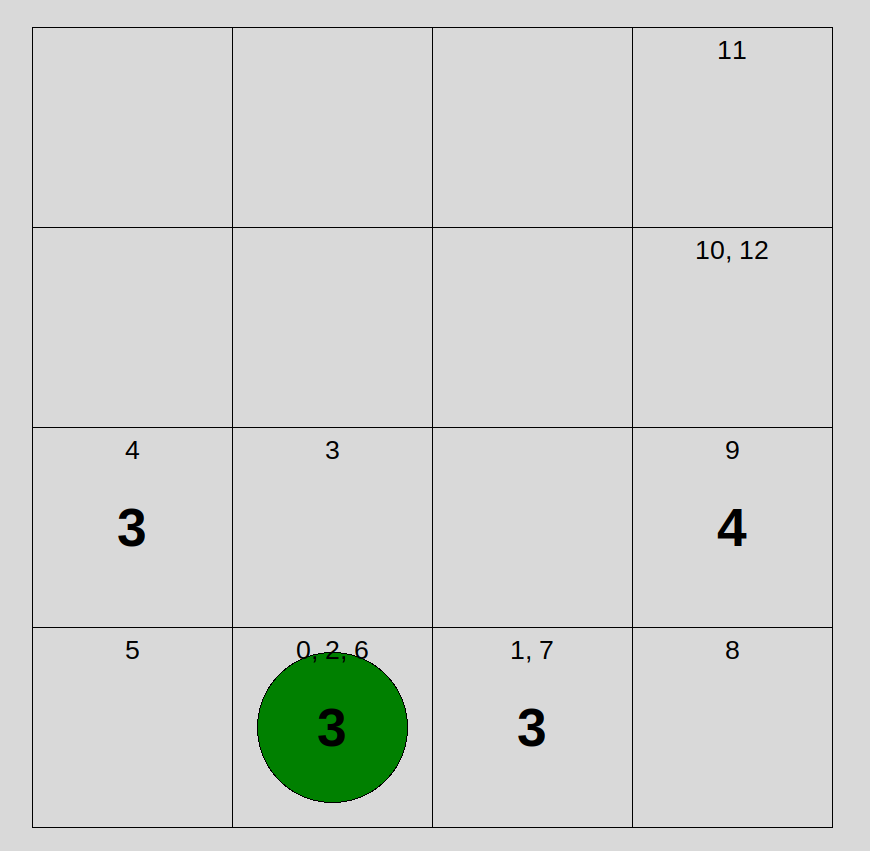
\includegraphics[width=0.8\textwidth]{aufgabe1_2_solution.png}
    \caption{Ein generariertes Strom-Rallye Spiel}
    \label{fig:loesung1}
\end{figure}
\newpage
\begin{classInformation}{PlayingFieldGenerator}
\addDescription{Die PlayingFieldGenerator- Klasse ist die einzige Klasse, des 2.Teils. Diese erzeugt ein zufälliges, lösbares Stromrallye Spiel}
\begin{classAttributes}
\addAttribute{-}{playing\_-field\_builder}{PlayingFieldBuilder}{baut das Spielfeld}
\addAttribute{-}{positions\_used}{HashSet[Position]}{Speichert alle Positionen an welchen bereits ein Objekt ist, damit nicht zwei Objekte an einem Ort sind. Das HashSet eignet sich dafür, da es nur $O(1)$ Zeit benötigt.}
\end{classAttributes}

\begin{classMethods}
\addMethod{+}{create\_-solveable\_-playing\_field}{PlayingField}{Die Methode erzeugt ein lösbares Spielfeld}
\end{classMethods}

\end{classInformation}
\subsection{Aufgabe 3}
\subsubsection{Beschreibung}
Bei Aufgabe 3, geht es darum einen Weg zu finden welcher moglichst kurz, aber auch moglichst seltenes Abbiegen beinhaltet.
So soll man fur ein Strasennetz einen Weg finden welcher am wenigsten Abbiegungen enthält aber auch maximal $n\%$ langer ist, als der kurzetser Weg, wobei $n$ vom User manuell eingegeben wird.
\textcite{bwinfSpielfeld}


\subsubsection{Losungsidee}
Als erstes wandele ich das Strasennetz in einen Graphen um.
Dabei wird eine Kreuzung zu einem Knoten in dem erstellten Graphen.
Eine Strase wird zu einer Kante in dem Graphen.
Die Lange des Weges werden die Kosten der Kante.


%%% da muss noch viel gemacht werden!!!
\begin{figure}[h!]
    \centering
    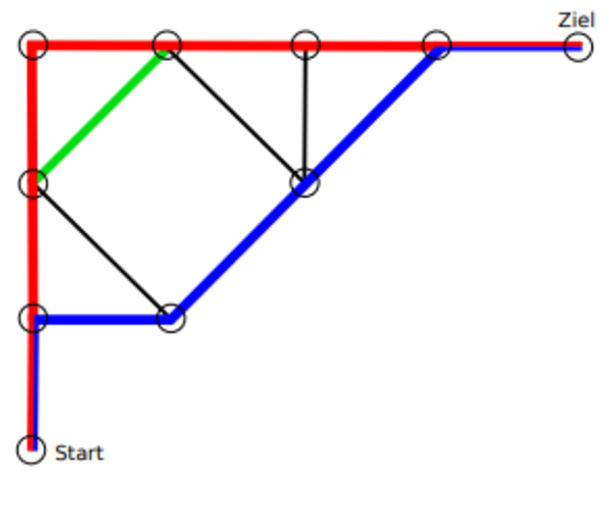
\includegraphics[width=0.6\textwidth]{aufgabe3.pdf}
    \caption{Straßennetz, rot ist der Weg mit den wenigsten Abkürzungen}
    \label{fig:abbiegen}
\end{figure}

\par
Dann finde ich in diesem Graphen alle moglichen Wege vom Start zum Ziel.
Nur Wege ohne Zyklen, also nur Wege welche einen Knoten maximal 1 mal besuchen. Da Wege welche einen Knoten mehrmals besuchen, langer sein mussen.
Es macht nie Sinn fur Bilal einen Knoten doppelt zu besuchen.
Auserdem wurde es sonst unendliche viele mogliche Wege geben, was es unlosbar machen wurde.

\begin{figure}[h!]
    \centering
    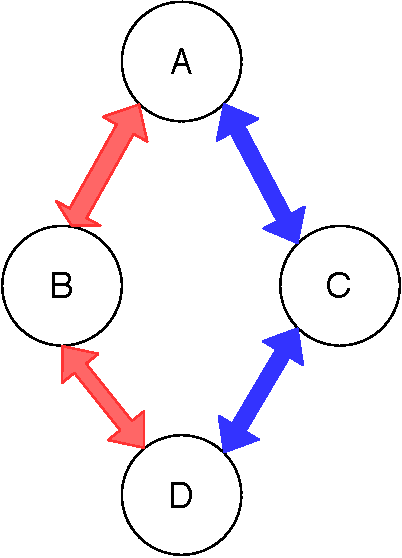
\includegraphics[width=0.6\textwidth]{small_example_graph.pdf}
    \caption{Graph}
    \label{fig:abbiegen}
\end{figure}
\par
Es gibt von A nach D, die möglichen Wege A -> B -> D und A -> C -> D.


\par
Um alle moglichen Wege zu finden. Verwende ich die Tiefen Suche, von jedem mit Tiefen Suche gefundenen Knoten wird wieder tiefen Suche ausgefuhrt.
Wenn man auf einen Knoten stost, welcher das Ziel ist oder schon besucht wurde wird abgebrochen.

\par
Algorithmus:
\begin{figure}[h!]
    \centering
    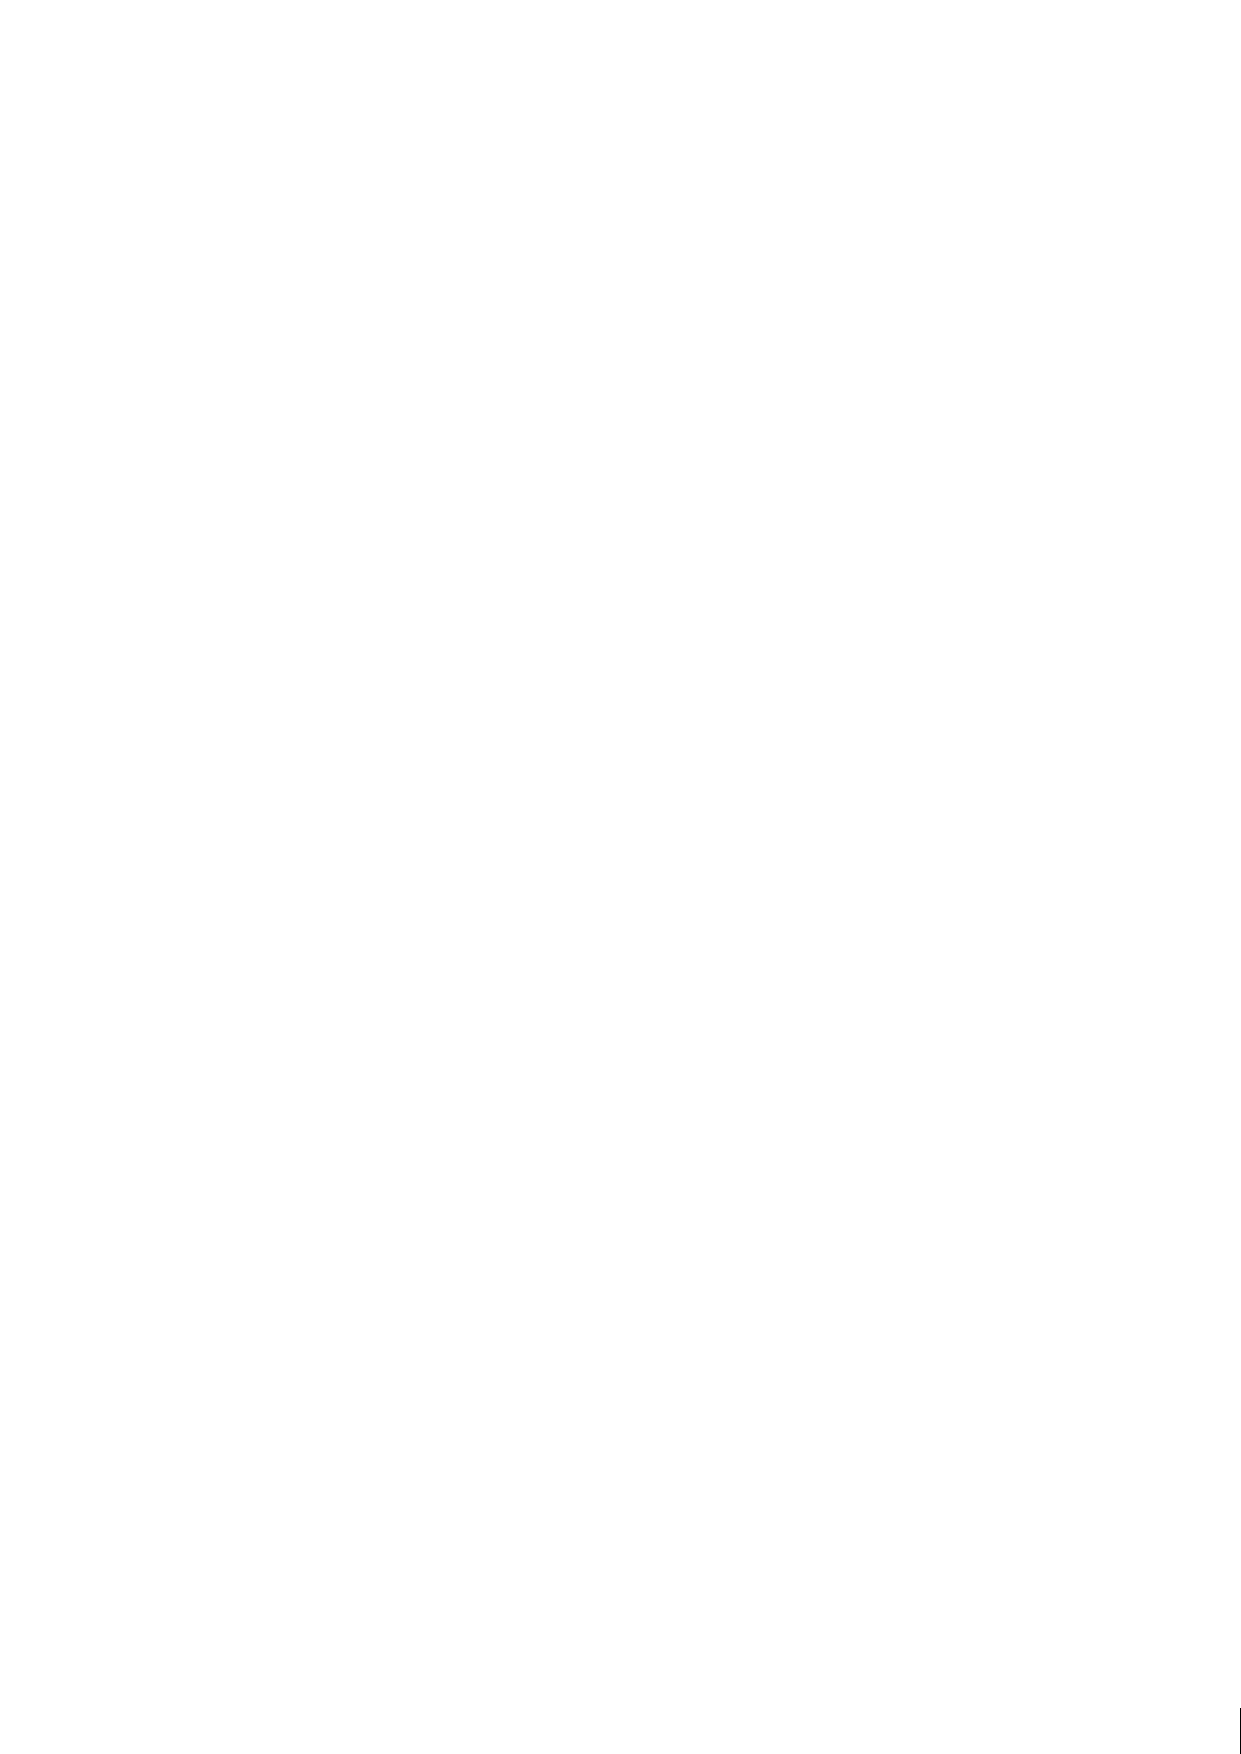
\includegraphics[width=0.4\textwidth]{PAP_find_path.pdf}
    \caption{Programmablaufplan um den besten Weg zu finden}
    \label{fig:pap3}
\end{figure}

\newpage
\subsubsection{Abbiegungen finden}
Wenn man vom Knoten $k$ zum Knoten $k'$ geht und beide eine Position im 2-dimensionalen Raum haben, $kp$ und $kp'$, respektiv.
Dann bewegt man sich in Richtung $kp'-kp$ wenn man sich von  $k$ zu $k'$ bewegt. Also bewegt man sich in Richtung des Richtungsvektors $r$. Wenn man nun von $k'$ zu $k''$ geht, in Richtung $r'$.
Ist dies ein Abbiegen, wenn $r != r'$.
Durch diese Definition ist auch denkbar, die Aufgabe fur ein Strasennetz durchzufuhren in welchem, es kompliziertere Kreuzungen gibt.
\begin{figure}[h!]
    \centering
    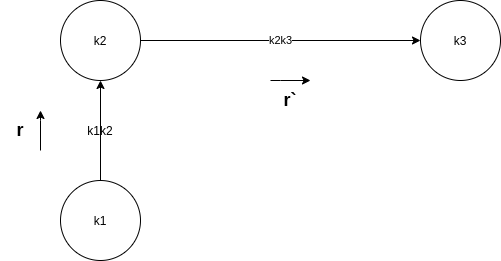
\includegraphics[width=0.6\textwidth]{AbbiegenBWinf.png}
    \caption{}
    \label{fig:abbiegen}
\end{figure}


Die $visited_nodes$ \ref{fig:pap3}, sind ein unsortiertes HashSet (Erklarung in Kapitel \ref{sec:HashSet}) , da dieses konstante Zeit braucht um ein Element zu suchen(herauszufinden ob es existiert) und um ein Element hinzuzufugen.
Dieses speichert keine Duplikate, was auch perfekt fur uns passt, da jeder Knoten nur maximal einmal besucht werden soll.
\par
Daraufhin sortiere ich alle Wege nach der Lange des Weges. So konnen mit binarer Suche sehr schnell alle Wege gefunden werden, welche kurz genug sind. Nun bestimme ich mit linearer Suche, den Weg mit den wenigsten Abkurzungen.
\subsubsection{HashSet}\label{sec:HashSet}
Ein HashSet speichert eine Menge an Daten. Dabei hat es die besondere Eigenschaft, dass es keine Duplikate speichert, jedes Element ist entweder einmal oder keinmal drinnen.

Zur Implementierung wird intern ein Array gespeichert. Fur jedes neu eingefugt Element, wird in das Array, an der Stelle des Hashwertes  $True$ eingetragen.
Der Hashwert eines Elements wird mit Hilfe einer Hashfunktion ermittelt.

Um zu prufen ob ein Element im HashSet ist, wird die gleiche Hashfunktion wie beim eintragen verwendet. Nun wird nachgeschaut, ob an dieser Stelle True oder False. Wenn True, dann ist dieses Element enthalten, wenn False dann nicht. Um ein ELement zu loschen, wird der Wert im Array auf False gesetzt.

Auf Grund dieser Implementierung, ist das HashSet unsortiert.

Der Vorteil gegenuber einer Liste besteht darin, dass es nur $O(1)$ Zeit benotigt um zu prufen ob ein Element enthalten ist, sowie $O(1)$, um ein Element hinzuzufugen.

\subsubsection{Besten Pfade speichern}
Speichern der besten Pfade zu jedem Knoten(Kreuzung) in einer HashMap.
Am Anfang, kennen wir nur den Weg zum Startknoten.
Nun updaten wir fur alle Nachbarn des Startknoten die Map Eintrage. Dann von diesen Nacharn wieder ... und so weiter.
Ein Knoten wird nur "betrachtet", wenn ein besserer Weg zu ihm gefunden wurde. So das er weniger Abbiegungen hat oder schneller ist.
\subsubsection{HashMap}
Eine HashMap speichert key-value Paare.
Man kann fur einen Schlussel(key) einen entsprechenden Wert finden.
Neue Key value Paare konnen in die HashMap einzutragen.

Die HashMap Implementierung, funktioniert folgendermasen. Es wird ein Array erzeugt.
Nun wird fur einen neu eingefugten Key Value Paar. Der Hashwert des Keys mit einer Hashfunktion ermittelt, am entsprechenden Index des Hashwertes, wird nun der Value eingetragen.

Um in einer Hashmap um fur einen Schlussel einen Wert zu finden wird nur konstante Zeit benotigt, genauso wie ein Wert-Schlussel Paar einzufugen.


\subsubsection{Zielfuhrenden Pfade zuerst}
In einer Priority Queue (Binary Heap), die zielfuhrendsten Pfade speichern, die am nahesten am Ziel dran sind, bis jetzt den Weg mit den wenigsten Abbiegungen haben.
Aus dieser Priority Queue immer das nachste Element hinaus nehmen und fur dieses die Wege zu den Nachbarn updaten. Neu gefudene Pfade in die Priority Queue einfugen.

\subsubsection{Priority Queue Binary Heap}
In einer Priority QUeue wird eine Menge an ELementen gespeichert. Dabei wird fur jedes Element auch eine Prioritat gespeichert.
Die Piority Quee, besitzt die FUnktion, das Element mit der geringsten oder maximalen Prioritat zuruck zugeben. Je nachdem, ob es eine Min-Heap oder Max-Heap ist.
Fur Priority Queues, gibt es verschiedene Implementierungen. Unter Anderem auch die Linked List, aber dabei ist die Performance nicht sonderbar gut. Da es O(n) ZEit braucht um das kleinste Element zu finden.
\textcite{skienaPriorityQueue}

Die Implementierung, welche ich gewahlt habe ist die Binary Heap, da in diese sehr schnell neue Elemente eingefugt werden und auch das kleinste Element gefunden werden kann.

\subsubsection{Binary Heap}
Die Binary Heap, ist ein Binary Tree, mit ein paar Beschrankungen.
Also jeder Knoten hat bis zu 2 Kind Knoten.
Anders als beim Tree, ist bei der Heap, der Eltern Knoten immer kleiner als die Kind Knoten.
Neue Knoten werden in der tiefsten Ebene moglichst weit links eingefugt.


\subsubsection{Fruhzeitiges Abbrechen}
Abbrechen, wenn der Zielknoten, einer der Nachbarknoten ist. Dann macht es nur Sinn den Zielknoten zu besuchen.

\subsubsection{Zielweg speichern}
Wenn ein Weg schlechter ist, als der beste Weg zum Ziel, bzw. wenn der beste Weg, welcher von einem Knoten zum Ziel gefunden werden kann, schlechter ist als der bis jetzt beste Weg zum Zielknoten, dann braucht man diesen Knoten nicht weiter zuverfolgen, sondern kann diesen loschen.

 
\subsubsection{Analyse}
Vom ersten Knoten werden neue Knoten zu allen Nachbar Knoten gefunden, von diesen wieder zu den Nachbar Knoten, ein Knoten wird aber nur besucht wenn ein besserer Knoten zu ihm gefunden wurde. Da die besseren Knoten durch die Priority Queue zuerst besucht werden und diese dann fur Knoten schnell sehr gute Wege finden. Werden viele Knoten nicht oft besucht werden. Ein Knoten kann bessere Wege zu den Nachbarn finden, diese konnen den Knoten nicht nochmal besuchen, da sie an diesem schon waren.

\section{Fazit}
\section{Anhang}
\subsectio{Bundeswettbewerb Informatik Aufgaben}



\subsection{Beispiel3}
\subsubsection{Eingabe}
\texttt{ \\
14 \\
3,5,9 \\
3 \\
6,4,4 \\
5,12,10 \\
6,2,5 \\
}
\subsubsection{Losung}
\begin{figure}[h]
    \centering
    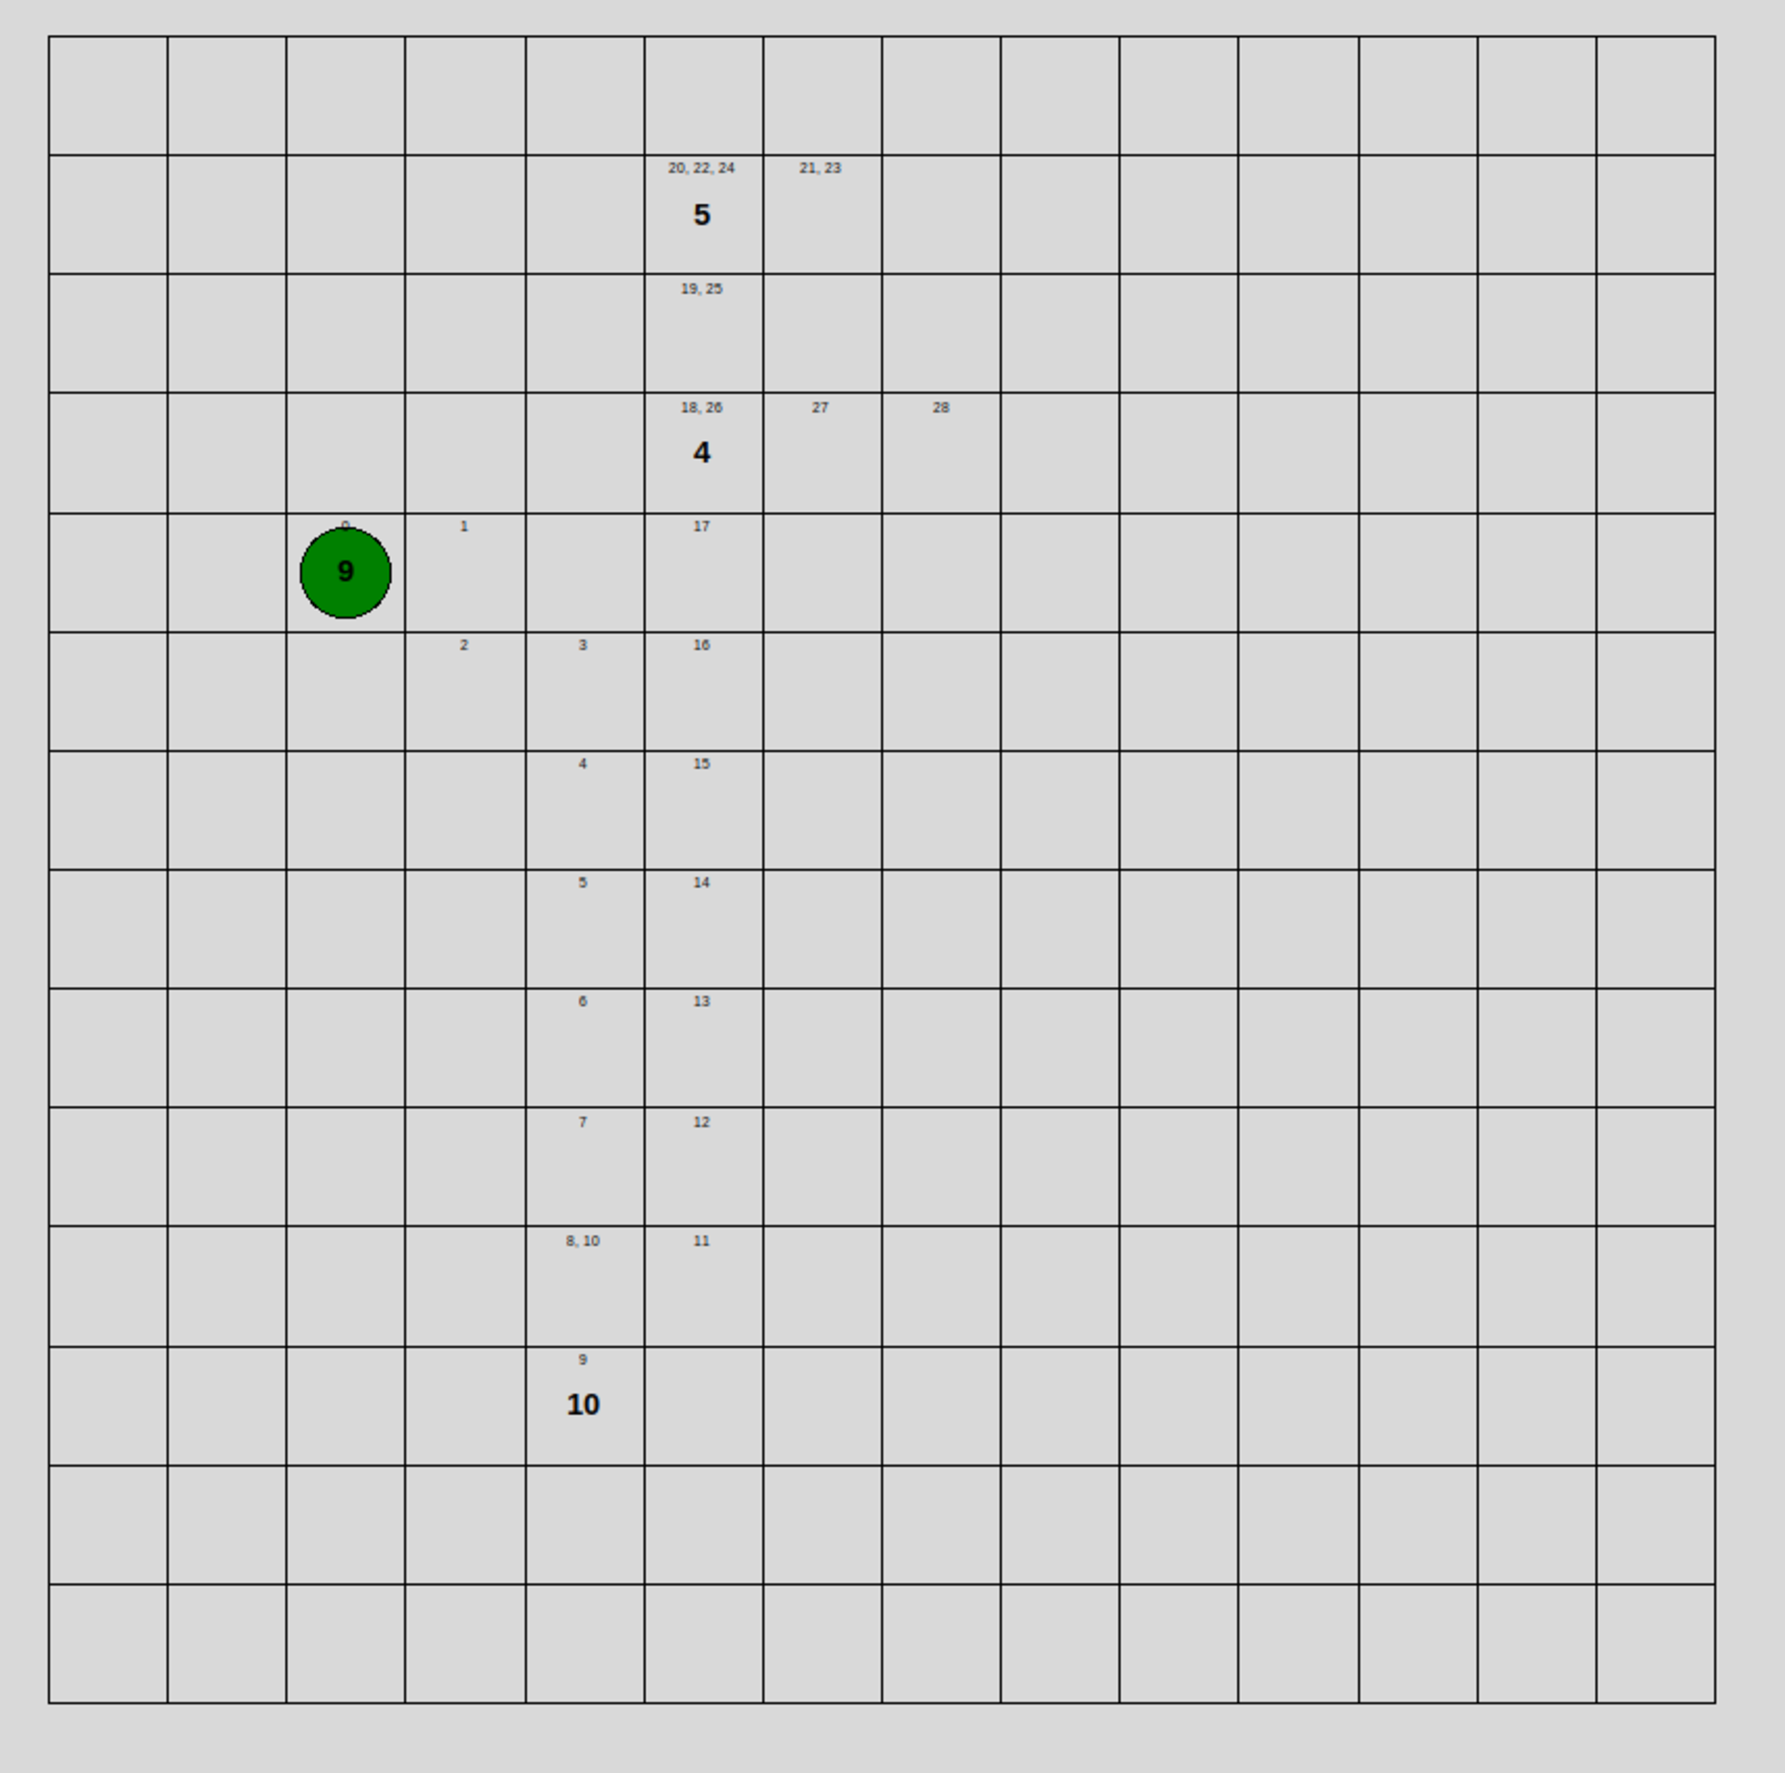
\includegraphics[width=\textwidth]{solution3.pdf}
    \caption{Losung des BWinfs Stromrallye Spiels Beispiel 3}
    \label{fig:loesung3}
\end{figure}

\subsection{Beispiel4}
\subsubsection{Eingabe}
\texttt{ \\
100 \\
40,25,20 \\
0 \\
}
\subsubsection{Losung}
\begin{figure}[h]
    \centering
    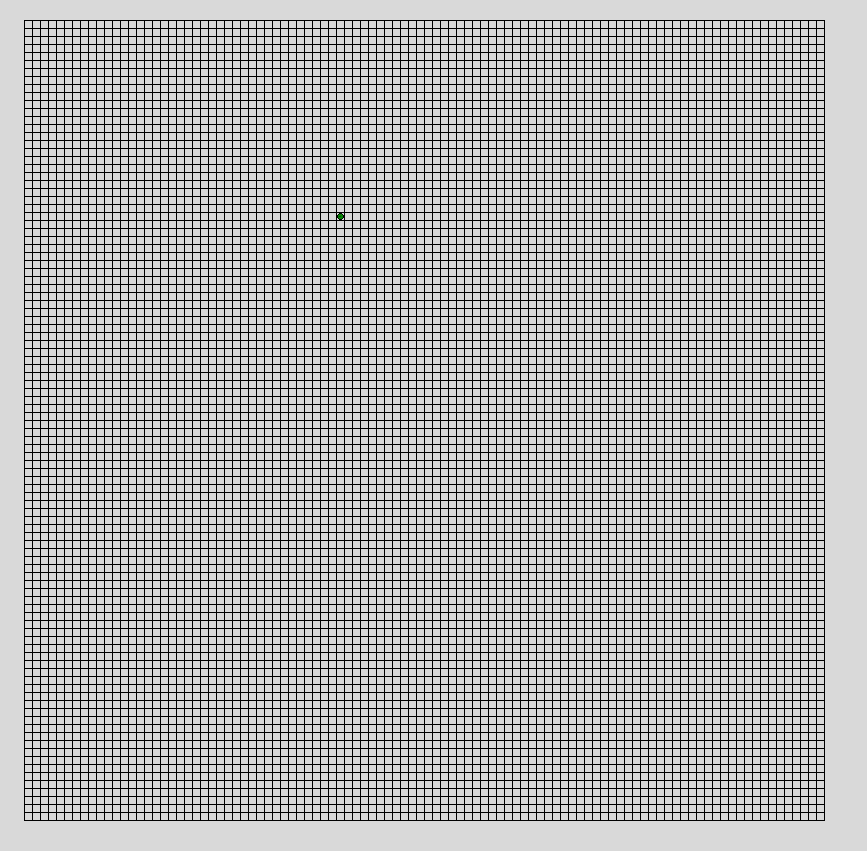
\includegraphics[width=0.8\textwidth]{solution4.png}
    \caption{Losung des BWinfs Stromrallye Spiels Beispiel 4}
    \label{fig:loesung4}
\end{figure}
Da auf Grund der Grose wenig zu erkennen ist.
Hier heran gezoomt.
\begin{figure}[h]
    \centering
    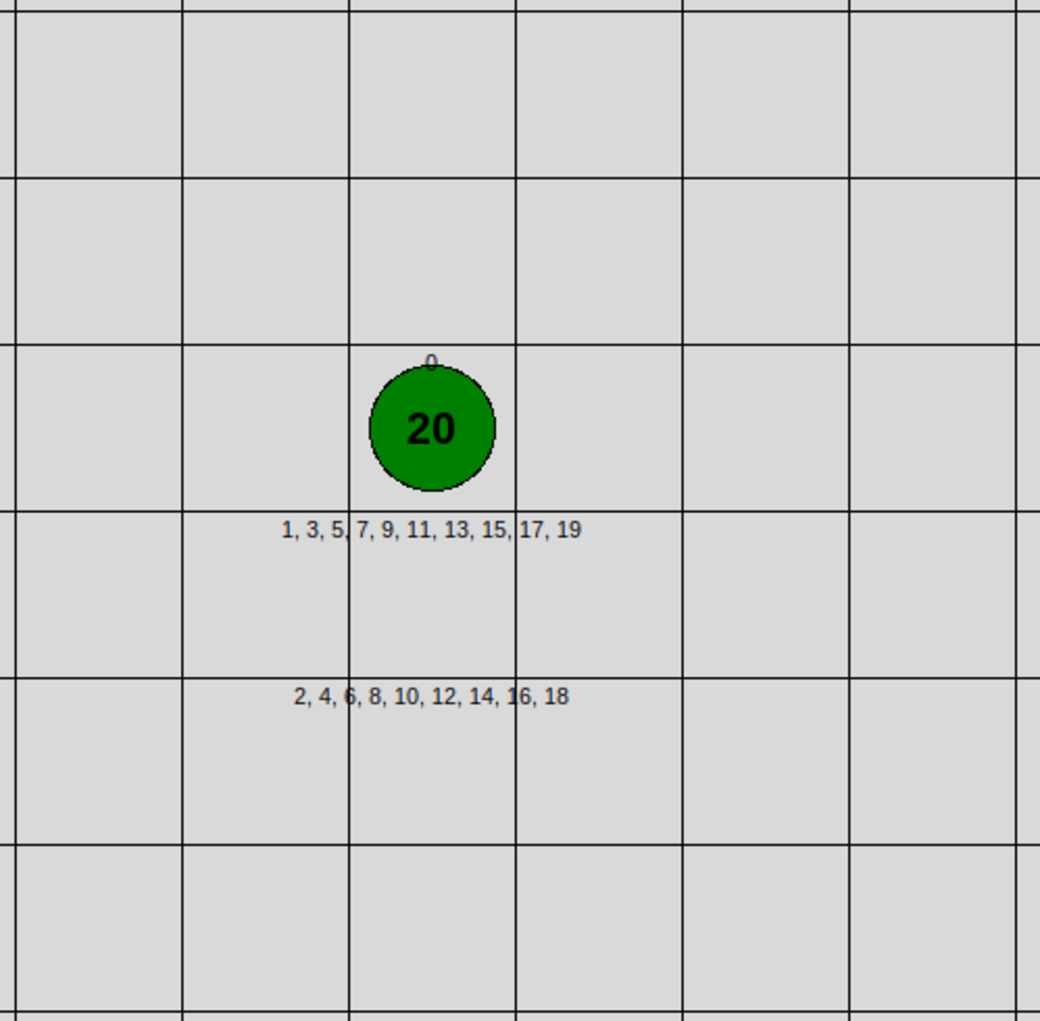
\includegraphics[width=\textwidth]{solution_4_zoomed.pdf}
    \caption{Losung des BWinfs Stromrallye Spiels Beispiel 4 heran gezoomt}
    \label{fig:loesung4_zoomed}
\end{figure}


\section{Quellen}


\printbibheading
\printbibliography[type=online,heading=subbibliography,title={Digital}]
\printbibliography[nottype=online,heading=subbibliography,title={Bucher}]



\section{Erklarung uber die selbstandige Anfertigung der Arbeit}
Hiermit erklare ich, dass ich die vorliegende Arbeit selbststandig und ohne fremde Hilfe verfasst, alle aus anderen Werken wortlich oder sinngemas entnommenen Stellen und Abbildungen unter Angabe der Quelle als Entlehnung kenntlich gemacht und keine anderen Hilfsmittel als die angegebenen verwendet habe. \\
\Ort, \today \space \Name


\end{document}
